% =====================================================================================
% AutoPareto: CAMERA-READY (NeurIPS 2026 AutoMLR workshop, poster)
% Source of truth: this file + generated/camera_ready/* (see camera_ready/BUILD.md).
% Revision 4 (2026-11-14): reader-first restructure answering the four reviews (Area Chair, NDEA,
% tKK, wwml): plain-language abstract and opening, "How AutoPareto works", Opus decision lineage
% (cr_v3.py), inference-mechanism figure, compact results table, chronological selection funnel,
% reproducibility levels.  Numbers come from generated/camera_ready/cr_macros*.tex.  Do NOT run
% refresh_paper.sh.  Part 2 passages drafted or changed for the camera-ready are wrapped in
% \humanauthor[ID]{...}; the workshop expects Part 2 to be human-written.
% Pre-revision-4 source: camera_ready/source_before_revision4/main.tex.
% Revision 6 (2026-11-15): AutoResearch explainer, revised abstract, provisional Part 2 restructure
% (P2-02..P2-17 "r6" tags), disclosure in three roles, checkboxes removed. Pre-revision-6 source:
% camera_ready/source_before_revision6/main.tex.
% Revision 7 (2026-11-15): two named phases (original / extended; Pair-A defined once), all eight approaches,
% main-text comparison figure (cr_comparison, raw-record Opus throughput), ~32x headline, appendix approach
% table. Part 2 received name substitutions only (listed in camera_ready/CHANGELOG_CAMERA_READY.md).
% Pre-revision-7 source: camera_ready/source_before_revision7/main.tex.
% Revision 9 (2026-11-15): one candidate comparison (cr_compare), three research histories (cr_lineage3), one
% downstream table, Opus decode path (cr_inference2), names GPT A22/A24/A25 everywhere (analysis/cr_r9.py).
% Part 2 received name substitutions only (camera_ready/CHANGELOG_CAMERA_READY.md). Pre-revision-9 source:
% camera_ready/source_before_revision9/main.tex.
% =====================================================================================
\documentclass{article}
\usepackage[dblblindworkshop,final]{neurips_2026}
\workshoptitle{Workshop for Autonomous ML Research}
\usepackage[utf8]{inputenc}
\usepackage[T1]{fontenc}
\usepackage{hyperref,url,booktabs,amsfonts,amsmath,microtype,xcolor,graphicx,float}
\usepackage{array}
\usepackage{capt-of}
\usepackage{needspace}
\usepackage[most]{tcolorbox}
\setlength{\textfloatsep}{7pt plus 2pt minus 2pt}
\setlength{\intextsep}{5pt plus 2pt minus 2pt}
\setlength{\floatsep}{5pt plus 2pt minus 2pt}
\setlength{\abovecaptionskip}{3pt}
\setlength{\belowcaptionskip}{0pt}
\renewcommand{\topfraction}{.92}
\renewcommand{\bottomfraction}{.7}
\renewcommand{\textfraction}{.06}
\renewcommand{\floatpagefraction}{.85}
\hypersetup{pdfauthor={},pdftitle={AutoPareto: Auditing Fixed-Time Autonomous Transformer Search with Matched-Exposure Verification},colorlinks=true,citecolor=blue,linkcolor=blue,urlcolor=blue}
% Generated by analysis/cr_tables.py from paper/camera_ready/data/cr_stats.json. Do not edit by hand.
\newcommand{\CRDecodeRatio}{1.99}
\newcommand{\CRDecodeRatioSeeds}{1.97, 1.96, 2.03}
\newcommand{\CRDecodeRatioMin}{1.96}
\newcommand{\CRDecodeRatioMax}{2.03}
\newcommand{\CRParamReduction}{41.7}
\newcommand{\CRMemoryReduction}{35.1}
\newcommand{\CRAPQSpeed}{383.0}
\newcommand{\CRARSpeed}{192.9}
\newcommand{\CRAPQHeld}{1.1418}
\newcommand{\CRARHeld}{1.0998}
\newcommand{\CRAPQParams}{29.36}
\newcommand{\CRARParams}{50.33}
\newcommand{\CRAPQMem}{162.9}
\newcommand{\CRARMem}{250.9}
\newcommand{\CRAPQKV}{1.992}
\newcommand{\CRARKV}{3.984}
\newcommand{\CRHeldDiff}{+0.042}
\newcommand{\CRHeldDiffAbs}{0.042}
\newcommand{\CRHeldDiffFour}{+0.0420}
\newcommand{\CRHeldCI}{[+0.030, +0.054]}
\newcommand{\CRHeldCIFour}{[+0.0297, +0.0544]}
\newcommand{\CRHeldCILo}{0.030}
\newcommand{\CRHeldCIHi}{0.054}
\newcommand{\CRValDiff}{+0.045}
\newcommand{\CRValDiffFour}{+0.0451}
\newcommand{\CRValCIFour}{[+0.0415, +0.0486]}
\newcommand{\CRHeldSeeds}{+0.0387, +0.0477, +0.0397}
\newcommand{\CRValSeeds}{+0.0440, +0.0467, +0.0445}
\newcommand{\CRFixedDiff}{$-$0.0067}
\newcommand{\CRFixedDiffThree}{$-$0.007}
\newcommand{\CRFixedCIFour}{[$-$0.0130, $-$0.0003]}
\newcommand{\CRFixedSeeds}{$-$0.0054, $-$0.0051, $-$0.0096}
\newcommand{\CRDiscGap}{$-$0.0017}
\newcommand{\CRPooledSD}{0.0022}
\newcommand{\CRMaxHeldSD}{0.0060}
\newcommand{\CRBaseSeedEffect}{0.024}
\newcommand{\CRSeedFortyTwoAP}{1.0940}
\newcommand{\CRSeedFortyTwoAR}{1.0950}
\newcommand{\CRSeedFortyTwoTPE}{1.0977}
\newcommand{\CRSeedFortyTwoMOTPE}{1.0981}
\newcommand{\CRSeedFortyTwoSpread}{0.0041}
\newcommand{\CROptMin}{0.0014}
\newcommand{\CROptMax}{0.0087}
\newcommand{\CRGapTwoMax}{0.0003}
\newcommand{\CRGapFiveMax}{0.0021}
\newcommand{\CRTokenSpreadMax}{18.7}
\newcommand{\CRExpOneThreeSixDisc}{251.8}
\newcommand{\CRExpOneThreeSixRerunLo}{209.7}
\newcommand{\CRExpOneThreeSixRerunHi}{220.5}
\newcommand{\CRExpOneZeroNineBPB}{1.0940}
\newcommand{\CRExpOneZeroNineTokens}{84.1}
\newcommand{\CRExpSixEightTokens}{88.9}
\newcommand{\CRAPAttempts}{75}
\newcommand{\CRCatArch}{32}
\newcommand{\CRCatOptimizer}{21}
\newcommand{\CRCatOptimization}{10}
\newcommand{\CRCatBatching}{8}
\newcommand{\CRCatSchedule}{4}
\newcommand{\CRStepNineteenTwenty}{0.0020}
\newcommand{\CRStepTwentyTwentyTwo}{0.00009}
\newcommand{\CRAnineBPB}{1.1068}
\newcommand{\CRAtenBPB}{1.1054}
\newcommand{\CRAnineDec}{324.7}
\newcommand{\CRAtenDec}{291.0}
\newcommand{\CRAtwentyfiveDec}{408.4}
\newcommand{\CRFrontierN}{6}
\newcommand{\CRPanelBudget}{201{,}326{,}592}
\newcommand{\CRARTokRatio}{2.28}
\newcommand{\CRAPQTokRatio}{1.28}
\newcommand{\CRFixedSixtyFive}{1.1017}
\newcommand{\CRFixedSixtyEight}{1.1014}
\newcommand{\CRBLiMPLower}{51}
\newcommand{\CRBLiMPTied}{1}
\newcommand{\CRBLiMPHigher}{15}
\newcommand{\CRBLiMPConfigs}{67}
\newcommand{\CRNCrossChecked}{118}
\newcommand{\CRSessionLo}{0.0035}
\newcommand{\CRSessionHi}{0.0070}
\newcommand{\CRHeldValOffLo}{0.053}
\newcommand{\CRHeldValOffHi}{0.069}
\newcommand{\CRCorrBLiMPHeld}{-0.969}
\newcommand{\CRCorrBLiMPDepth}{0.717}
\newcommand{\CRAPQARCE}{36.91}
\newcommand{\CRAPQPIQA}{58.29}
\newcommand{\CRAPQLAMBADA}{21.50}
\newcommand{\CRAPQBLiMP}{72.02}
\newcommand{\CRARARCE}{36.50}
\newcommand{\CRARPIQA}{58.67}
\newcommand{\CRARLAMBADA}{20.44}
\newcommand{\CRARBLiMP}{74.56}
\newcommand{\CRARCESE}{1.0}

% Generated by analysis/cr_v2.py from paper/camera_ready/data/cr_v2.json. Do not edit by hand.
\newcommand{\CREOneHeldA}{+0.0385}
\newcommand{\CREOneHeldB}{+0.0396}
\newcommand{\CREOneHeldC}{+0.0415}
\newcommand{\CREOneMatchedLo}{+0.038}
\newcommand{\CREOneMatchedHi}{+0.042}
\newcommand{\CREOneMatchedLoAbs}{0.038}
\newcommand{\CREOneMatchedHiAbs}{0.042}
\newcommand{\CREOneTimeHeld}{$-$0.0022}
\newcommand{\CREOneTimeHeldThree}{$-$0.002}
\newcommand{\CREOneTimeHeldCI}{[$-$0.020, +0.016]}
\newcommand{\CREOneTimeHeldLo}{$-$0.020}
\newcommand{\CREOneTimeHeldHi}{+0.016}
\newcommand{\CREOneTimeVal}{$-$0.0044}
\newcommand{\CREOneTimeValThree}{$-$0.004}
\newcommand{\CREOneTimeValCI}{[$-$0.012, +0.004]}
\newcommand{\CREOneTimeHeldWins}{1}
\newcommand{\CREOneContrast}{+0.0031}
\newcommand{\CREOneContrastCI}{[$-$0.0017, +0.0078]}
\newcommand{\CREOnePairs}{9}
\newcommand{\CREOneMaxSD}{0.0045}
\newcommand{\CREOneReplDiff}{$-$0.0005}
\newcommand{\CREOneReplCI}{[$-$0.0120, +0.0110]}
\newcommand{\CREOneTokAP}{158.1}
\newcommand{\CREOneTokAR}{88.0}
\newcommand{\CREOneTokRatio}{1.80}
\newcommand{\CREOneHistWelch}{+0.0023}
\newcommand{\CREOneResamples}{27}
\newcommand{\CREOneExposure}{$-$0.041}
\newcommand{\CREOneExposureCI}{[$-$0.042, $-$0.039]}
\newcommand{\CREOneArch}{+0.040}
\newcommand{\CREOneArchCI}{[+0.023, +0.056]}
\newcommand{\CREOneSched}{$-$0.001}
\newcommand{\CREOneExposureVal}{$-$0.047}
\newcommand{\CREOneArchVal}{+0.043}
\newcommand{\CREOneRho}{1.81}
\newcommand{\CREOneK}{1.79}
\newcommand{\CREOneKCI}{[1.29, 2.28]}
\newcommand{\CREOneKVal}{1.70}
\newcommand{\CRFixedTokAR}{88.5}
\newcommand{\CRFixedTokAPQ}{156.9}
\newcommand{\CRAgBaseBPB}{1.1999}
\newcommand{\CRAgBaseTok}{85.5}
\newcommand{\CRAgBaseMem}{337}
\newcommand{\CRAgBaseDecode}{149}
\newcommand{\CRAgEtoERef}{146}
\newcommand{\CRAgEtoERefRep}{143}
\newcommand{\CRAgPrefillRef}{7.5}
\newcommand{\CROpStableRepeats}{6}
\newcommand{\CROpRepeats}{9}
\newcommand{\CROpAttempts}{27}
\newcommand{\CROpValid}{25}
\newcommand{\CROpValidFrozen}{23}
\newcommand{\CROpUncertain}{7}
\newcommand{\CROpBestBPB}{1.0962}
\newcommand{\CROpBestAttempt}{23}
\newcommand{\CROpBestFrozen}{1.0962}
\newcommand{\CROpBestTwentyTwo}{1.0969}
\newcommand{\CROpBestTwentyTwoAttempt}{20}
\newcommand{\CROpBestSeven}{1.0995}
\newcommand{\CROpLateGain}{0.0033}
\newcommand{\CROpUpdLo}{1,504}
\newcommand{\CROpUpdHi}{1,514}
\newcommand{\CROpLateDone}{19}
\newcommand{\CROpLateInf}{11}
\newcommand{\CROpMaxTok}{232}
\newcommand{\CROpTokLo}{197}
\newcommand{\CROpTokHi}{198}
\newcommand{\CROpTokRatio}{2.3}
\newcommand{\CROpDecodeLo}{30.9}
\newcommand{\CROpDecodeHi}{31.8}
\newcommand{\CROpEtoELo}{5.2}
\newcommand{\CROpEtoEHi}{5.3}
\newcommand{\CROpPrefillLo}{140}
\newcommand{\CROpPrefillHi}{143}
\newcommand{\CROpMemLo}{97}
\newcommand{\CROpMemHi}{113}
\newcommand{\CROpHeldLo}{1.158}
\newcommand{\CROpHeldHi}{1.161}
\newcommand{\CROpARHeld}{1.100}
\newcommand{\CROpAPQHeld}{1.142}
\newcommand{\CROpTokFrac}{98}
\newcommand{\CROpAdapterAttempt}{10}
\newcommand{\CROpPreAdapterDecode}{2.6}
\newcommand{\CROpPreAdapterPrefill}{6}
\newcommand{\CROpAdapterDecode}{8.6}
\newcommand{\CROpAdapterPrefill}{81}
\newcommand{\CROpDLambadaLo}{+0.049}
\newcommand{\CROpDLambadaHi}{+0.061}
\newcommand{\CROpDBlimpLo}{+0.059}
\newcommand{\CROpDBlimpHi}{+0.070}
\newcommand{\CROpDHeldLo}{0.088}
\newcommand{\CROpDHeldHi}{0.091}
\newcommand{\CREOneHours}{4.76}
\newcommand{\CREOneTputAR}{288.2--289.7k}
\newcommand{\CREOneTputAP}{520.7--524.9k}
\newcommand{\CREZeroTputAR}{287.0k}
\newcommand{\CREZeroTputAP}{521.8k}
\newcommand{\CROpFrontierFrozen}{A21, A23, A24}
\newcommand{\CROpFrontierExtended}{A23, A24, A27}
\newcommand{\CRCxAttempts}{22}
\newcommand{\CRCxValid}{22}
\newcommand{\CRCxUncertain}{1}
\newcommand{\CRCxBestBPB}{1.1016}
\newcommand{\CRCxBestAttempt}{14}
\newcommand{\CRCxBestTok}{126.6}
\newcommand{\CRCxMaxTok}{175}
\newcommand{\CRCxBestDecode}{1.32}
\newcommand{\CRCxMaxDecode}{1.58}
\newcommand{\CRCxMaxPrefill}{27}
\newcommand{\CRMTRuns}{10}
\newcommand{\CRMTPairs}{9}
\newcommand{\CRMTDLo}{+0.059}
\newcommand{\CRMTDHi}{+0.061}
\newcommand{\CRMTDLoAbs}{0.059}
\newcommand{\CRMTDHiAbs}{0.061}
\newcommand{\CRMTCIMin}{+0.051}
\newcommand{\CRMTHolm}{0.002}
\newcommand{\CRMTDAPLo}{+0.017}
\newcommand{\CRMTDAPHi}{+0.019}
\newcommand{\CRMTDAPCIMin}{+0.004}
\newcommand{\CRMTValLo}{+0.062}
\newcommand{\CRMTValHi}{+0.065}
\newcommand{\CRMTHeldLo}{1.158}
\newcommand{\CRMTHeldHi}{1.160}
\newcommand{\CRMTARHeld}{1.099}
\newcommand{\CRMTAPHeld}{1.141}
\newcommand{\CRMTTpsLo}{657}
\newcommand{\CRMTTpsHi}{658}
\newcommand{\CRMTTpsAR}{289}
\newcommand{\CRMTTpsAP}{523}
\newcommand{\CRMTRhoLo}{2.27}
\newcommand{\CRMTRhoHi}{2.28}
\newcommand{\CRMTKBound}{2.27}
\newcommand{\CRMTKExtLo}{2.38}
\newcommand{\CRMTKExtHi}{2.46}
\newcommand{\CRMTPostLo}{+0.001}
\newcommand{\CRMTPostHi}{+0.003}
\newcommand{\CRMTPostCILo}{$-$0.005}
\newcommand{\CRMTPostCIHi}{+0.012}
\newcommand{\CRMTBlimpLo}{0.034}
\newcommand{\CRMTBlimpHi}{0.038}
\newcommand{\CRMTBlimpLoPts}{3.4}
\newcommand{\CRMTBlimpHiPts}{3.8}
\newcommand{\CRMTKAPQ}{1.86}
\newcommand{\CRMTDrift}{$-$0.0010}
\newcommand{\CRMTDriftAbs}{0.0010}
\newcommand{\CRMTParamsLo}{22.0}
\newcommand{\CRMTParamsHi}{26.2}
\newcommand{\CRIARuns}{39}
\newcommand{\CRIAUnstable}{5}
\newcommand{\CRIATotalLo}{30.7}
\newcommand{\CRIATotalHi}{30.8}
\newcommand{\CRIAGraphLo}{11.2}
\newcommand{\CRIAGraphHi}{11.7}
\newcommand{\CRIAFusionLo}{2.7}
\newcommand{\CRIAFusionHi}{2.8}
\newcommand{\CRIAJointLo}{15.6}
\newcommand{\CRIAJointHi}{16.7}
\newcommand{\CRIAInteractLo}{0.51}
\newcommand{\CRIAInteractHi}{0.52}
\newcommand{\CRIAAttnLo}{1.29}
\newcommand{\CRIAAttnHi}{1.29}
\newcommand{\CRIARingLo}{1.05}
\newcommand{\CRIARingHi}{1.05}
\newcommand{\CRIAArchLo}{1.85}
\newcommand{\CRIAArchHi}{1.97}
\newcommand{\CRIATotalMed}{31}
\newcommand{\CRIAEtoEMed}{5.3}
\newcommand{\CRIAEtoELo}{5.2}
\newcommand{\CRIAEtoEHi}{5.4}
\newcommand{\CRIAGraphEtoELo}{1.9}
\newcommand{\CRIAGraphEtoEHi}{2.0}
\newcommand{\CRIAFusionEtoEHi}{1.07}
\newcommand{\CRIAPrefillLo}{131}
\newcommand{\CRIAPrefillHi}{138}
\newcommand{\CRIAPrefillNGLo}{3.7}
\newcommand{\CRIAPrefillNGHi}{4.3}
\newcommand{\CRIAPrefillBase}{7.3}
\newcommand{\CRIACapture}{97}
\newcommand{\CRIAKVOp}{3.6}
\newcommand{\CRIAKVLin}{7.5}
\newcommand{\CRIABaseDecode}{149}
\newcommand{\CRIABaseDecodeLo}{145}
\newcommand{\CRIABaseDecodeHi}{153}
\newcommand{\CRIAKernBase}{625}
\newcommand{\CRIALaunchBase}{618}
\newcommand{\CRIAKernEager}{290}
\newcommand{\CRIAKernFused}{78}
\newcommand{\CRIALaunchNG}{75}
\newcommand{\CRIALaunchGraph}{2}
\newcommand{\CRMTHours}{2.61}
\newcommand{\CRIAHours}{3.10}
\newcommand{\CRBenchSDMax}{2.3}
\newcommand{\CRBenchSDMed}{0.7}

% Generated by analysis/cr_v3.py. Do not edit by hand.
\newcommand{\CRCxAbsDecode}{193}
\newcommand{\CRFiveMTDAPHiAbs}{0.019}
\newcommand{\CRFiveMTDAPLoAbs}{0.017}
\newcommand{\CRFivePilotNA}{85.9}
\newcommand{\CRFivePilotNB}{35.7}
\newcommand{\CRFivePilotNC}{47.2}
\newcommand{\CRFivePilotRatioHi}{2.2}
\newcommand{\CRFivePilotRatioLo}{1.7}
\newcommand{\CRFivePilotTA}{50.3}
\newcommand{\CRFivePilotTB}{16.3}
\newcommand{\CRFivePilotTC}{24.6}
\newcommand{\CRIAAbsHi}{4{,}595}
\newcommand{\CRIAAbsLo}{4{,}581}
\newcommand{\CROpAbsHi}{4{,}592}
\newcommand{\CROpAbsLo}{4{,}570}
\newcommand{\CROpAbsSpreadPct}{0.5}
\newcommand{\CROpAbsTwentyFour}{4{,}578}
\newcommand{\CROpAbsTwentySeven}{4{,}592}
\newcommand{\CROpAbsTwentyThree}{4{,}570}
\newcommand{\CROpCampHi}{31.4}
\newcommand{\CROpCampLo}{30.5}
\newcommand{\CROpCampTwentyThree}{30.8}
\newcommand{\CRPTwoBaseHi}{151}
\newcommand{\CRPTwoBaseLo}{135}
\newcommand{\CRThreeCaptureMs}{132}
\newcommand{\CRThreeDecBase}{852}
\newcommand{\CRThreeDecOpus}{28}
\newcommand{\CRThreeDecX}{30.8}
\newcommand{\CRThreeElevenTok}{193}
\newcommand{\CRThreeEtoEX}{5.3}
\newcommand{\CRThreeFiveParams}{26.2}
\newcommand{\CRThreeFiveTok}{196}
\newcommand{\CRThreeInfOnly}{11}
\newcommand{\CRThreeLateGain}{0.0033}
\newcommand{\CRThreeLateValid}{19}
\newcommand{\CRThreeOneTok}{85}
\newcommand{\CRThreeOneUpd}{323}
\newcommand{\CRThreePreBase}{7}
\newcommand{\CRThreePreNoFusion}{96}
\newcommand{\CRThreePreOpus}{136}
\newcommand{\CRThreeSevenUpd}{1{,}474}
\newcommand{\CRThreeSixWorse}{0.021}
\newcommand{\CRThreeTotBase}{859}
\newcommand{\CRThreeTotOpus}{163}
\newcommand{\CRThreeTwelveTok}{149}
\newcommand{\CRThreeTwentyFiveTok}{108}

% Generated by analysis/cr_r8.py. Do not edit by hand.
\newcommand{\CREightTrainRatio}{1.81}
\newcommand{\CREightDecodeRatio}{1.99}
\newcommand{\CREightMemRed}{35}
\newcommand{\CREightARTrain}{289}
\newcommand{\CREightAPTrain}{523}
\newcommand{\CREightOpTrainLo}{657}
\newcommand{\CREightOpTrainHi}{658}
\newcommand{\CREightARDecode}{193}
\newcommand{\CREightAPDecode}{383}
\newcommand{\CREightCxBest}{1.1016}
\newcommand{\CREightCxBestX}{1.32}
\newcommand{\CREightCxMaxX}{1.58}
\newcommand{\CREightCxFirstX}{0.96}
\newcommand{\CREightCxBatchGain}{0.062}
\newcommand{\CREightOpSevenVal}{1.0995}
\newcommand{\CREightOpSixWorse}{0.021}
\newcommand{\CREightOpTenX}{8.6}
\newcommand{\CREightOpFourteenX}{16.8}
\newcommand{\CREightOpEighteenX}{24.7}
\newcommand{\CREightOpNineteenX}{29.6}
\newcommand{\CREightOpTwentyTwoX}{32.0}
\newcommand{\CREightOpSevenX}{2.47}
\newcommand{\CREightOpEightMemDrop}{52}
\newcommand{\CREightAPOneGain}{0.107}
\newcommand{\CREightAPEightWorse}{0.061}
\newcommand{\CREightAPQDisc}{313}
\newcommand{\CREightARFail}{31}
\newcommand{\CREightAPBaseDisc}{164}
\newcommand{\CREightARFour}{1.189}
\newcommand{\CREightARSix}{1.099}
\newcommand{\CREightOpTwentySevenX}{31.5}
\newcommand{\CREightOpTwentyFourParams}{22.0}
\newcommand{\CREightBenchSDMax}{2.3}
\newcommand{\CREightBenchSDMed}{0.7}

% Generated by analysis/cr_r9.py. Do not edit by hand.
\newcommand{\CRNineTrainRatio}{1.81}
\newcommand{\CRNineOpTrainRatioLo}{2.27}
\newcommand{\CRNineOpTrainRatioHi}{2.27}
\newcommand{\CRNineGptDecX}{1.9}
\newcommand{\CRNineOpMemRed}{66}
\newcommand{\CRNineBaseMem}{337}
\newcommand{\CRNineOpMemTwentyThree}{113}
\newcommand{\CRNineOpMemTwentySeven}{99}
\newcommand{\CRNineArcGptPanel}{36.9}
\newcommand{\CRNineArcARPanel}{36.5}
\newcommand{\CRNineLambGptPanel}{21.5}
\newcommand{\CRNineLambARPanel}{20.4}
\newcommand{\CRNineArcSix}{36.7}
\newcommand{\CRNineArcARSix}{36.2}
\newcommand{\CRNinePiqaOpus}{58.4}
\newcommand{\CRNinePiqaARSix}{58.1}
\newcommand{\CRNineLambOpus}{22.3}
\newcommand{\CRNineLambARSix}{21.9}
\newcommand{\CRNineBenchSDMax}{2.3}
\newcommand{\CRNineBenchSDMed}{0.7}
\newcommand{\CRNineEtoEX}{5.3}
\newcommand{\CRNineARHeldSix}{1.0995}
\newcommand{\CRNineGptHeldSix}{1.1410}

\newcommand{\CRSixDecodeLo}{4,579}
\newcommand{\CRSixDecodeHi}{4,591}
\newcommand{\CRSixSpeedLo}{31.4}
\newcommand{\CRSixSpeedHi}{32.1}
\newcommand{\CRSixEtoELo}{663}
\newcommand{\CRSixEtoEHi}{672}
\newcommand{\CRSixEtoEXLo}{4.6}
\newcommand{\CRSixEtoEXHi}{4.6}
\newcommand{\CRSixPrefillLo}{163}
\newcommand{\CRSixPrefillHi}{165}
\newcommand{\CRSixBasePrefill}{7.3}
\newcommand{\CRSixBaseDecode}{145}
\newcommand{\CRSixBaseEtoE}{146}
\newcommand{\CRSixBaseEtoEms}{880}
\newcommand{\CRSixOpusEtoEms}{192}
\newcommand{\CRSixGptBestDecode}{373}
\newcommand{\CRSixARHeld}{1.099}
\newcommand{\CRSixARFixed}{1.157}
\newcommand{\CRSixFrontTokens}{AR-ref, NSGA-II, TPE, GPT A22, Opus A27, Opus A24}
\newcommand{\CRSixFrontFixed}{GPT A22, Opus A27, Opus A24}
\newcommand{\CRSixModels}{13}
\newcommand{\CRSixRuns}{39}
\newcommand{\CRSixGptDecRatio}{1.8}
\newcommand{\CRSixGptMemRed}{28}
\newcommand{\CRSixGptMem}{243}
\newcommand{\CRSixARMem}{337}
\newcommand{\CRSixOpMemLo}{96}
\newcommand{\CRSixOpMemHi}{110}
\newcommand{\CRSixOpDecDms}{28}
\newcommand{\CRSixBaseDecDms}{873}
\newcommand{\CRSixGptTokD}{+0.042}
\newcommand{\CRSixGptTokCI}{[+0.029, +0.054]}
\newcommand{\CRSixGptTimeD}{$-$0.002}
\newcommand{\CRSixGptTimeCI}{[$-$0.020, +0.016]}
\newcommand{\CRSixOpTwThreeTokD}{+0.059}
\newcommand{\CRSixOpTwThreeTokCI}{[+0.051, +0.066]}
\newcommand{\CRSixOpTwThreeTimeD}{+0.002}
\newcommand{\CRSixOpTwThreeTimeCI}{[$-$0.002, +0.006]}
\newcommand{\CRSixOpTwFourTokD}{+0.061}
\newcommand{\CRSixOpTwFourTokCI}{[+0.052, +0.070]}
\newcommand{\CRSixOpTwFourTimeD}{+0.003}
\newcommand{\CRSixOpTwFourTimeCI}{[$-$0.011, +0.017]}
\newcommand{\CRSixOpTwSevenTokD}{+0.059}
\newcommand{\CRSixOpTwSevenTokCI}{[+0.053, +0.064]}
\newcommand{\CRSixOpTwSevenTimeD}{+0.002}
\newcommand{\CRSixOpTwSevenTimeCI}{[$-$0.004, +0.008]}
\newcommand{\CRSixTpeTokD}{+0.021}
\newcommand{\CRSixTpeTokCI}{[+0.010, +0.032]}
\newcommand{\CRSixTpeTimeD}{$-$0.001}
\newcommand{\CRSixTpeTimeCI}{[$-$0.011, +0.010]}
\newcommand{\CRSixNsgaTokD}{+0.014}
\newcommand{\CRSixNsgaTokCI}{[+0.004, +0.025]}
\newcommand{\CRSixNsgaTimeD}{+0.014}
\newcommand{\CRSixNsgaTimeCI}{[+0.005, +0.022]}
\newcommand{\CRSixRsTokD}{+0.023}
\newcommand{\CRSixRsTokCI}{[+0.009, +0.036]}
\newcommand{\CRSixRsTimeD}{+0.001}
\newcommand{\CRSixRsTimeCI}{[$-$0.007, +0.009]}
\newcommand{\CRSixTokWorseCount}{12}
\newcommand{\CRSixTokDLo}{0.014}
\newcommand{\CRSixTokDHi}{0.088}
\newcommand{\CRSixTimeResolved}{4}
\newcommand{\CRSixFrontEveryTok}{AR-ref, TPE, GPT A22, Opus A27 and Opus A24}
\newcommand{\CRSixFrontTwoTok}{NSGA-II and Opus A23}
\newcommand{\CRSixFrontEveryTime}{Opus A24}
\newcommand{\CRSixUnstableRuns}{11}
\newcommand{\CRSixUnstableMaxDev}{10}
\newcommand{\CRSixSeedCVMax}{6}
\newcommand{\CRSixBracketLo}{126}
\newcommand{\CRSixBracketHi}{154}
\newcommand{\CRSixCorrectRuns}{39}
\newcommand{\CRSixHardMismatches}{0}
\newcommand{\CRSixNearTies}{83}
\newcommand{\CRSixMaxLogitErr}{0.32}
\newcommand{\CRSixFixedMaxExcess}{0.87}
\newcommand{\CRSixGptTrainRatio}{1.81}
\newcommand{\CRSixOpTrainRatio}{2.3}
\newcommand{\CRSixArcBest}{GPT A24}
\newcommand{\CRSixArcBestVal}{38.1}
\newcommand{\CRSixArcAR}{36.2}
\newcommand{\CRSixPiqaBest}{Random Search}
\newcommand{\CRSixPiqaBestVal}{59.1}
\newcommand{\CRSixPiqaAR}{58.1}
\newcommand{\CRSixLambBest}{Opus A27}
\newcommand{\CRSixLambBestVal}{22.3}
\newcommand{\CRSixLambAR}{21.9}
\newcommand{\CRSixBlimpBest}{AR-ref}
\newcommand{\CRSixBlimpBestVal}{74.5}
\newcommand{\CRSixBlimpAR}{74.5}
\newcommand{\CRSixLeadRunnerMax}{1.3}
\newcommand{\CRSixArcBestOverAR}{1.9}
\newcommand{\CRSixRhoWiki}{0.98}
\newcommand{\CRSixRhoBlimp}{-0.96}
\newcommand{\CRSixRhoSciq}{$-$0.58}
\newcommand{\CRSixRhoNearMax}{0.41}
\newcommand{\CRSixLmSDMax}{7.5}
\newcommand{\CRSixAnchorSpeedMax}{2.1}
\newcommand{\CRSixAnchorDecodeMax}{6}
\newcommand{\CRSixAnchorPreA}{167}
\newcommand{\CRSixAnchorPreB}{146}
\newcommand{\CRSixAccSDMax}{1.6}
\newcommand{\CRSixFrontMeanOnlyTok}{NSGA-II}
\newcommand{\CRSixFrontMeanOnlyTime}{GPT A22 and Opus A27}
\newcommand{\CRSixStableShiftMax}{5.4}
\newcommand{\CRSixUnstableSeedSix}{8}
\newcommand{\CRSixOpDecSpread}{0.3}
\newcommand{\CRSixFlagBaseDrift}{11}
\newcommand{\CRSixFlagCandDrift}{8}
\newcommand{\CRSixFlagCV}{4}
\newcommand{\CRSixFlagDrift}{10}
\newcommand{\CRSixFlagCVOnly}{1}
\newcommand{\CRSixFlagCVOnlyName}{GPT A25 seed 6}
\newcommand{\CRSixCancelled}{7}
\newcommand{\CRSixOpusWinIQR}{0.04}
\newcommand{\CRSixRefWinIQR}{7.8}
\newcommand{\CRSixBlockFlags}{6}
\newcommand{\CRSixBlockRuns}{8}
\newcommand{\CRSixBlockStart}{20:31}
\newcommand{\CRSixBlockEnd}{21:02}
\newcommand{\CRSixRestFlags}{5}
\newcommand{\CRSixRestRuns}{31}
\newcommand{\CRSixTokensChecked}{39,936}
\newcommand{\CRSixTokensAgree}{39,853}
\newcommand{\CRSixAgreePct}{99.8}
\newcommand{\CRSixNearTieMaxDeficit}{0.11}
\newcommand{\CRSixTimedEqual}{39}
\newcommand{\CRSixDecXVsBaseRecipe}{31.6}
\newcommand{\CRSixBonfTok}{8}
\newcommand{\CRSixBonfTokLost}{Random Search, TPE, NSGA-II and GPT A22}
\newcommand{\CRSixBonfTime}{1}
\newcommand{\CRSixBonfTimeKept}{the baseline}
\newcommand{\CRSixBonfT}{15.4}
\newcommand{\CRSixTimeWorseNames}{the baseline, MOTPE, NSGA-II and GPT A24}


% == Human-authorship markers (Part 2) ==
\newif\ifshowhumanmarkers \showhumanmarkersfalse
\definecolor{humanframe}{HTML}{B2412A}
\newcommand{\humantag}[1]{{\color{humanframe}\sffamily\scriptsize\bfseries HUMAN AUTHOR MUST REWRITE/VERIFY [#1]}\ }
\newtcolorbox{humanbox}{breakable,enhanced,colback=humanframe!4,colframe=humanframe,boxrule=0.4pt,arc=0pt,
  left=2pt,right=2pt,top=1pt,bottom=1pt,boxsep=0.5pt,before skip=3pt,after skip=3pt,parbox=false}
\newcommand{\humanauthor}[2][]{\ifshowhumanmarkers\begin{humanbox}\humantag{#1}#2\end{humanbox}\else #2\par\fi}
\newcommand{\humancaption}[1]{\ifshowhumanmarkers\humantag{#1}\fi}
\newcommand{\releasepending}{\ifshowhumanmarkers{\color{humanframe}\sffamily\scriptsize\bfseries[RELEASE PENDING]}\ \fi}
\newcommand{\authortodo}[1]{{\color{humanframe}[#1]}}

\title{AutoPareto: Auditing Fixed-Time Autonomous Transformer Search\\with Matched-Exposure Verification}
\author{Rami Alobaidy\\ \texttt{rameonix@gmail.com}}
\begin{document}
\maketitle
\begin{abstract}
Autonomous research agents can design and optimize machine learning systems, but the goals we give them shape what they discover. We introduce AutoPareto, a multi-objective research framework built on Andrej Karpathy's autoresearch, in which coding agents modify a Transformer's architecture, its training procedure and, in a later campaign, its inference code. Rather than optimizing language modelling quality alone, AutoPareto scores quality, generation speed and memory, and every candidate trains for the same fixed GPU time. A faster program therefore also trains on more data. Across independent campaigns, agents from two model families discovered that smaller Transformers and smaller batches fit substantially more training into the same time. Starting from a model with 50 million parameters, AutoPareto found a 29-million-parameter design that decodes 1.8 times as fast as the quality-only autoresearch reference while using 28\% less inference memory. In a later campaign, a Claude Opus 5.5 agent found Transformers with 22 to 26 million parameters and rewrote their generation code with the established techniques of CUDA graph replay and kernel fusion, reaching approximately 32 times the scored decode-only throughput of the 50-million-parameter starting model, or 4.6 times for a whole generation. Pre-registered retraining on new random seeds showed why the time budget favoured these designs: they processed more data within the time limit but did not learn more from each training token. Autonomous agents can thus discover substantial system efficiencies, and the objectives and budgets we set shape which solutions they pursue.
\end{abstract}

\noindent\textbf{Keywords:} autonomous ML research; neural architecture search; Transformer efficiency; multi-objective optimization; reproducibility

\section{Autonomous research result}\label{partone}

\subsection{The question and the setup}\label{sec:question}\label{sec:brief}
\looseness=-1 In Karpathy's autoresearch \citep{autoresearch}, an AI agent repeatedly edits a language model's training program, trains each version for 300\,s on one GPU and keeps an edit only if the model improves; because the budget is time, a faster program also trains on more data. AutoPareto keeps this loop but scores quality, decoding speed and inference memory. \textbf{We ask what the agents discovered (\S\ref{sec:discover}), how (\S\ref{sec:search}), whether it holds up when every recipe is compared fairly (\S\ref{sec:verify}), and why Opus's recipes decode about 32$\times$ faster but generate only \CRSixEtoEXLo$\times$ faster (\S\ref{sec:inference}).}

\looseness=-1 \textbf{Terms.} Quality is \emph{bits per byte} (BPB) on unseen text, lower is better: agents saw \emph{validation BPB}; we confirm on \emph{held-out BPB} from a shard no agent saw (glossary: Appendix~\ref{app:glossary}).

\looseness=-1 \textbf{Setup.} Each candidate trains a small Transformer on web text (ClimbMix) for 300\,s on one NVIDIA A40, starting from 8 layers and 50.3M parameters.

\looseness=-1 \textbf{Search loop.} The agent edits only \texttt{train.py} (model, optimizer, training loop); a documented hook lets it add generation code, which the protected benchmark times (Appendix~\ref{app:access}). Each \emph{attempt} reads all earlier ones, picks a \emph{parent}, records a hypothesis and edits the file; protected code trains, measures and records it, failures included (Appendix Figure~\ref{fig:loop}). A recipe is on the \emph{Pareto frontier} if no other is at least as good on every objective and better on one.

\looseness=-1 \textbf{Eight approaches.} AutoPareto ran with GPT-5.6 (three campaigns of 25 attempts) and Claude Opus 5.5 (27 attempts, 25 valid, in a later harness; Part~\ref{parttwo}), against a quality-only AutoResearch agent (GPT-5.6) and five classical optimizers (Appendix~\ref{app:approaches}). \emph{GPT A22} is attempt 22 of GPT-5.6's seed-0 campaign; \emph{AR-ref} is AutoResearch's best recipe that passed the cache check. Campaigns differ in seed and harness, so we rank neither agents nor methods \citep[cf.][]{ferreira}.

\subsection{What did AutoPareto discover?}\label{sec:discover}

\begin{figure}[t]
\centering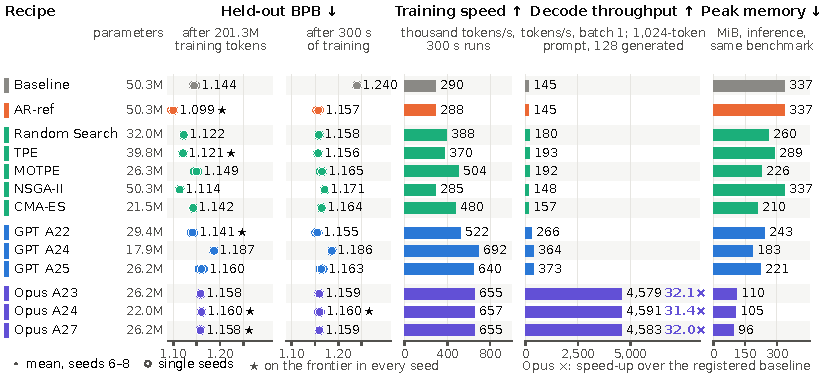
\includegraphics[width=\linewidth]{figures/cr_compare13.pdf}
\caption{All 13 recipes, seeds 6 to 8: held-out BPB after 201.3M tokens and after 300\,s, training speed (300\,s runs), and decode speed and peak memory on one inference benchmark and A40 (1{,}024 tokens in, 128 out, batch one). Stars: on the BPB--decode frontier in every seed. SDs: Table~\ref{tab:verify}.}\label{fig:overview}
\end{figure}

\looseness=-1 \textbf{Every agent found the same lever}: under a 300\,s budget smaller batches give more optimizer updates and smaller models more tokens. AutoResearch kept the 50.3M-parameter model (best held-out BPB at equal tokens). GPT A22 (4 layers, 29.4M) trains \CRSixGptTrainRatio$\times$ and decodes \CRSixGptDecRatio$\times$ as fast as AR-ref with \CRSixGptMemRed\% less memory; GPT A24 and A25 (17.9M, 26.2M) are faster still but worse.

\looseness=-1 \textbf{Opus also rewrote the inference engine.} Its 22 to 26M-parameter recipes train about \CRSixOpTrainRatio$\times$ as many tokens per second as AR-ref and decode \CRSixDecodeLo{} to \CRSixDecodeHi{} tokens per second, \CRSixSpeedLo$\times$ to \CRSixSpeedHi$\times$ its starting model, in \CRSixOpMemLo{} to \CRSixOpMemHi{} instead of \CRSixARMem\,MiB. Most of this comes from Opus's generation code, not its model (\S\ref{sec:inference}); the ten other recipes run the protected reference decoder, so the 32$\times$ compares engines as well as models and measures speed, not quality.

\subsection{How did the agents discover it?}\label{sec:search}\label{sec:compare}

\begin{figure}[t]
\centering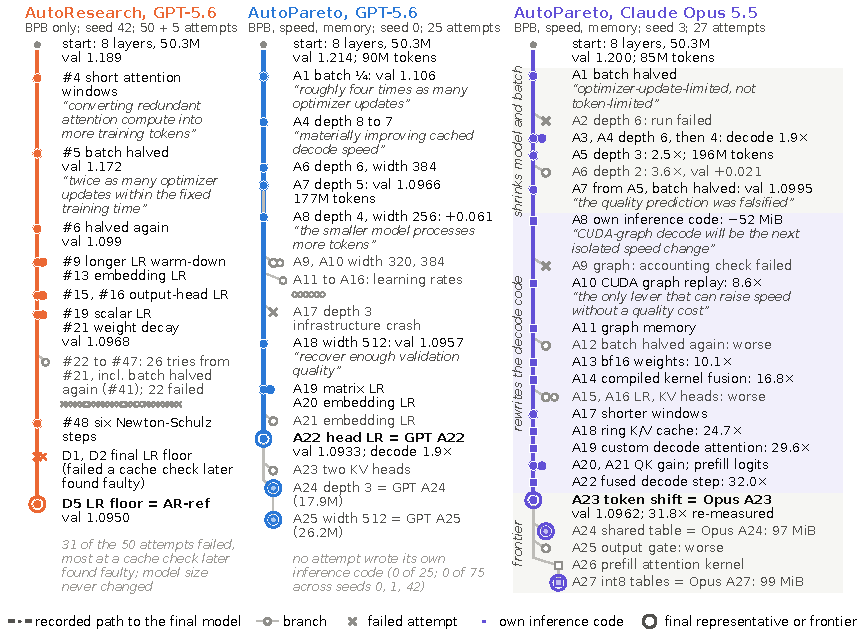
\includegraphics[width=\linewidth]{figures/cr_lineage3.pdf}
\caption{Three research histories in attempt order; lines join each attempt to its recorded parent; branches are abandoned or failed attempts (all: Figure~\ref{fig:histories}). Quotes: hypotheses recorded before each run. ``val'', tokens: validation BPB (comparable within a column) and training tokens of one 300\,s run. Speed-ups: search records over each starting model (final recipes re-timed in Figure~\ref{fig:overview}).}\label{fig:tracks}\label{fig:opus}
\end{figure}

\looseness=-1 \textbf{Three searches} (Figure~\ref{fig:tracks}). AutoResearch kept the model's size and tuned batch and learning rates (most failures: a faulty cache check, \S\ref{sec:interventions}). GPT-5.6 removed layers until A8 lost \CREightAPEightWorse, restored width 512 (A18) and tuned learning rates into GPT A22. Opus rewrote decoding from A8 and reached \CREightOpTwentyTwoX$\times$ by A22, while its \CRThreeLateValid{} valid attempts after A7 improved BPB by only \CRThreeLateGain{} in total.

\looseness=-1 \textbf{Why only Opus reached 32$\times$.} Both programs offered the same generation-code hook (Appendix~\ref{app:access}), and both agents first shrank the model, which made decoding about \CRNineGptDecX$\times$ faster in each campaign's search records (Opus by A4, GPT-5.6 with its selected A22). GPT-5.6 tied decode speed to model size, removing a layer for ``materially improving cached decode speed'' (A4), and wrote no inference code in any campaign. Opus hit a quality limit (``the quality prediction was falsified'', A7), identified kernel-launch overhead as the bottleneck and wrote that ``CUDA-graph replay is the only lever that can raise speed without a quality cost'' (A10). In these campaigns its inference-engine strategy was thus far more effective for decode speed. Each search ran once, under different harnesses (Part~\ref{parttwo}), so this is not evidence that either model is the better researcher.

\subsection{Comparing all recipes fairly}\label{sec:verify}
\looseness=-1 \textbf{One test for all 13 recipes.} To separate learning per token from speed, a final pre-registered test retrained all 13 recipes on new seeds 6 to 8 for 201.3M tokens and for 300\,s and timed each on one benchmark and A40 (Table~\ref{tab:verify}), reusing E1's and the Opus retraining's runs, checked by drift controls.

\begin{figure}[t]
\centering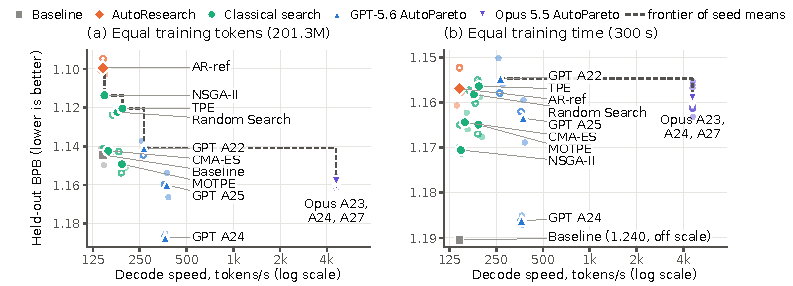
\includegraphics[width=\linewidth]{figures/cr_unified.pdf}
\caption{A two-objective projection: held-out BPB after (a) 201.3M tokens and (b) 300\,s against decode speed. AutoPareto also optimizes inference memory (Figure~\ref{fig:overview}, Table~\ref{tab:verify}). Large: means; small: seeds (rings: timing flag). Dashed: the means' frontier in these two objectives; \CRSixFrontMeanOnlyTok{} (a), \CRSixFrontMeanOnlyTime{} (b) are on it, not in every seed.}\label{fig:unifiedscatter}
\end{figure}

\looseness=-1 \textbf{Equal tokens: AR-ref learns most per token.} All \CRSixTokWorseCount{} other recipes are worse after 201.3M tokens, by \CRSixTokDLo{} to \CRSixTokDHi{} held-out BPB, in every seed, with every per-comparison 95\% interval above zero (\CRSixBonfTok{} of \CRSixTokWorseCount{} after a Bonferroni adjustment): GPT A22 by \CRSixGptTokD{} (as in E1), Opus's recipes by about 0.06. \textbf{Equal time: the leaders are not separated.} At 300\,s no recipe is resolved as better than AR-ref (GPT A22 \CRSixGptTimeD{} \CRSixGptTimeCI, Opus A27 \CRSixOpTwSevenTimeD{} \CRSixOpTwSevenTimeCI), which is not evidence of equality, and \CRSixTimeWorseNames{} are resolved as worse (only the baseline after adjustment). The pre-registered E1 (Appendix Figure~\ref{fig:e1}) explains GPT A22: it learns less per token than AR-ref at every token budget and seed but trains on \CREOneTokAP M tokens in 300\,s to AR-ref's \CREOneTokAR M; the two roughly cancel.

\looseness=-1 \textbf{No recipe wins everything} (Figures~\ref{fig:overview} and~\ref{fig:unifiedscatter}). At equal tokens \CRSixFrontEveryTok{} are on the frontier in every seed (the Opus recipes are \CRSixOpDecSpread\% apart in decode speed, so which of them is not resolved); at 300\,s the leaders' quality is not separated, so decode speed decides.

\looseness=-1 \textbf{Downstream tasks} (Appendix Tables~\ref{tab:verify} and~\ref{tab:lmeval}). AR-ref also leads BLiMP, narrowly, and WikiText perplexity, an independent language-modelling check that ranks recipes like held-out BPB ($\rho=\CRSixRhoWiki$). Smaller recipes lead ARC-Easy, PIQA and LAMBADA by at most \CRSixLeadRunnerMax{} points over the runner-up, within the seed SDs (up to \CRSixAccSDMax), not a ranking, and five of seven further tasks are near chance at this scale.

\looseness=-1 \textbf{Speed measurements.} Decode rates are medians over eight timed windows, each bracketed by baseline windows. \CRSixUnstableRuns{} of the 39 runs carry a timing flag, not a correctness failure (each passed the correctness check): their ratios to the baseline varied beyond the benchmark's stability limits (interquartile range 2\% of the median, coefficient of variation 5\%), and in all \CRSixFlagBaseDrift{} the baseline windows themselves varied by over 2\%. We report them as measured (rings in Figure~\ref{fig:unifiedscatter}); dropping them moves no mean by more than \CRSixStableShiftMax\% and leaves the means' Pareto frontier unchanged (Appendix~\ref{app:repro}). The 32$\times$ is far outside this noise; few-percent gaps between the slower recipes are not.

\subsection{Why do Opus's recipes decode 32$\times$ faster but generate only \CRSixEtoEXLo$\times$ faster?}\label{sec:inference}

\begin{figure}[t]
\centering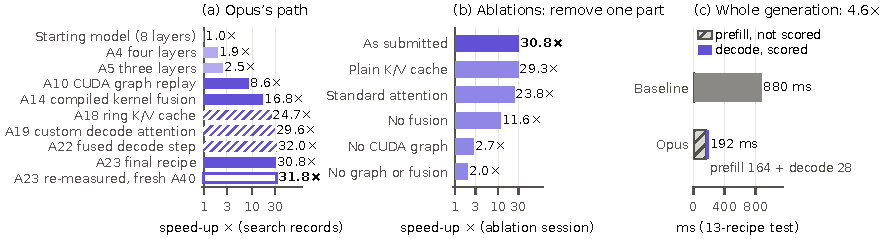
\includegraphics[width=\linewidth]{figures/cr_inference2.pdf}
\caption{Where Opus's speed comes from, one measurement per panel: (a) search records (steps accumulate; hatched: speed-uncertain); (b) pre-registered ablations of Opus A23, A24, A27 in one session (medians); (c) one whole generation in the 13-recipe test.}\label{fig:inference}
\end{figure}

\looseness=-1 Only \emph{decode} steps, each generating one token after the prompt is read (\emph{prefill}), are scored. At batch one they are dominated by CPU launches of GPU programs (\emph{kernels}), \CRIAKernBase{} per token at first; a \emph{CUDA graph} replays recorded kernels with one call and \emph{kernel fusion} merges them (\CRIAKernEager{} to \CRIAKernFused).

\looseness=-1 \textbf{An engine, not a better model} (Figure~\ref{fig:inference}a, b). The smaller model gave about \CRNineGptDecX$\times$ (A4) and Opus's engine most of the rest. Without the graph its recipes lose \CRIAGraphLo{} to \CRIAGraphHi$\times$, without fusion \CRIAFusionLo{} to \CRIAFusionHi$\times$, and without both they keep only \CRIAArchLo{} to \CRIAArchHi$\times$; the effects interact. Decode-only gains agree across sessions (\CRThreeDecX$\times$ in the ablations, \CRSixSpeedLo$\times$ to \CRSixSpeedHi$\times$ in the 13-recipe test).

\looseness=-1 \textbf{What the score does not time} (Figure~\ref{fig:inference}c). Opus records the graph inside the unscored prefill (``Prefill time rose from 6.4 ms to 81 ms'', A11). In the 13-recipe test prefill takes \CRSixPrefillLo{} to \CRSixPrefillHi{} ms against the baseline's \CRSixBasePrefill, while decoding falls from \CRSixBaseDecDms{} to \CRSixOpDecDms{} ms, so a whole generation is \CRSixEtoEXLo$\times$ faster (\CRThreeEtoEX$\times$ in the ablation session, mainly because its Opus prefill took \CRThreePreOpus{} ms).

\looseness=-1 \textbf{Correct outputs.} In all 39 runs, every generated token (8 prompts, positions 1{,}024 to 1{,}151, past Opus's ring-cache wrap) was checked against the recipe's uncached forward pass: \CRSixAgreePct\% of \CRSixTokensChecked{} match its greedy token, \CRSixNearTies{} are BF16 near-ties (within 0.25 logits), none is a hard mismatch.
\label{partoneend}

\clearpage
\section{System Design and Meta-Analysis}\label{parttwo}
% Part 2 must be human-written (workshop rule). Every passage drafted or changed for the
% camera-ready is wrapped in \humanauthor[P2-xx]{...}; camera_ready/PART2_HUMAN_AUTHORSHIP.md
% lists the facts, evidence paths and guidance for each ID.

\subsection{Agent and Harness}\label{sec:agent}
% P2-02: restructured in revision 6 by Claude; the author stated on 2026-11-15 that Part 2 is reviewed and approved. Revision 7 changed names only; the author approved them on 2026-11-15 (camera_ready/CHANGELOG_CAMERA_READY.md).
\humanauthor[P2-02 r6]{\looseness=-1 My role was to design the research framework, define the objectives, compute budgets and evaluation rules, and maintain the experimental infrastructure. The AI agents independently proposed hypotheses, modified Transformer architectures and training settings, and selected which candidates to explore. Three parts of the system should be kept apart. The \emph{model} proposes each change. The \emph{coding application} is the interface through which it reads files and runs commands. The \emph{protected runner} trains and evaluates the code, and the agent cannot change it.

\looseness=-1 \textbf{Original experiments.} Most original AutoPareto and AutoResearch experiments used GPT-5.6 (\texttt{gpt-5.6-sol}, high reasoning effort) through the Codex desktop application. For the first five attempts of the seed-42 campaign, the same model and setting were accessed through Cursor because Codex usage was nearly exhausted. In every case a protected experiment runner executed and evaluated the proposed code on the GPU. The agent started the runner over SSH, and isolation relied on the program's instructions plus hash checks: every protected file was hashed before and after each attempt, and any change outside \texttt{train.py} rejected the run.

\looseness=-1 \textbf{Extended experiments} (\S\ref{sec:pilot}). Here a controller called the agent and launched every run itself. The Codex arm ran the same GPT-5.6 model through Codex CLI, in a fresh container for every call that held five staged files. The Opus arm ran Claude Opus 5.5 through Claude Code, Anthropic's command-line coding agent, with file tools only and no shell. Both arms used the same prompts and output schemas, made two agent calls per attempt and could write only \texttt{train.py}. The Opus arm was isolated by command-line permissions, file modes and hash checks, tested by a canary before the campaign. No agent saw downstream results. Versions, timeouts and per-attempt attribution are in Appendix~\ref{app:repro}. Session logs survive for every campaign and stay private because they contain access credentials.}

\subsection{Tools}
% P2-03: restructured in revision 6 by Claude; the author stated on 2026-11-15 that Part 2 is reviewed and approved. Revision 7 changed names only; the author approved them on 2026-11-15 (camera_ready/CHANGELOG_CAMERA_READY.md).
\humanauthor[P2-03 r6]{\looseness=-1 All training and measurement ran in BF16 on NVIDIA A40 GPUs. Original discovery (July and August) did not log its environment, while the repository's lockfile pinned PyTorch 2.9.1. The matched-token verification (201.3M-token panel, E1, Opus retraining) used Python 3.10.18 with PyTorch 2.9.1. Extended runs and the inference ablations reusing their benchmark ran in a separate Python 3.12 runtime with PyTorch 2.8.0 (2.9.1 in the September pilot). Table~\ref{tab:env} records every era.}

\subsection{Research Loop}\label{sec:loop}
% P2-04: restructured in revision 6 by Claude; the author stated on 2026-11-15 that Part 2 is reviewed and approved. Revision 7 changed names only; the author approved them on 2026-11-15 (camera_ready/CHANGELOG_CAMERA_READY.md).
\humanauthor[P2-04 r6]{\looseness=-1 Each attempt follows the eight steps below. The agent acts in steps 2 and 8 and, in original runs, labels the outcome in step 7. Protected code does everything else (Appendix~\ref{app:repro} names the functions).\par
{\small\begin{enumerate}\setlength{\itemsep}{0pt}\setlength{\parskip}{0pt}\setlength{\topsep}{2pt}
\item \emph{Controller:} show the agent this campaign's records, the current frontier and the parent's source.
\item \emph{Agent:} return a hypothesis, the intended change, a change category, the chosen parent and a patch to \texttt{train.py}.
\item \emph{Controller:} validate. The parent must be on the current frontier (original) or parent-eligible in the same arm (extended). Protected files and the source must match their SHA-256 hashes, and only \texttt{train.py} may change.
\item \emph{Controller:} train under the contract, 300\,s or, in the extended fixed-token arm, $N^\star$ counted tokens.
\item \emph{Controller:} verify the checkpoint, measure validation BPB, check that cached decoding matches a full recomputation, and measure decode throughput and peak allocated memory.
\item \emph{Controller:} append an immutable record of the hypothesis, patch, hashes, metrics and any failure text. A failure still uses up the attempt.
\item \emph{Controller and agent:} update the archive. In the original experiments a completed candidate was retained unless another completed candidate or the registered same-seed baseline dominated it on raw BPB, decode speed and memory, with no noise margin. The agent labelled each outcome, and the runner rejected any label that disagreed with this rule.
\item \emph{Agent:} choose the next parent among the retained (original) or parent-eligible (extended) records.
\end{enumerate}}
\looseness=-1 Without a noise margin the archive keeps noise-level trade-offs. In GPT A22's campaign A9 and A10 build the same model, yet A10 was retained. In the extended experiments every quality-valid record was parent-eligible even when its speed was uncertain.}

\subsection{Human Interventions}\label{sec:interventions}
% P2-06: restructured in revision 6 by Claude; the author stated on 2026-11-15 that Part 2 is reviewed and approved. Revision 7 changed names only; the author approved them on 2026-11-15 (camera_ready/CHANGELOG_CAMERA_READY.md).
% Revision 10: factual update from the 13-recipe test, approved by the author on 2026-11-18 (camera_ready/PART2_REVISION10_PROPOSED.md).
\humanauthor[P2-06 r6]{\looseness=-1 I chose the objectives, the 300-second contract, the matched-exposure design, the recipes for the panel, E1, the Opus tests and the 13-recipe test, the comparators and the interpretation. I made or approved each intervention below, and AI coding assistants carried out several of them at my instruction. None of them counts as autonomous agent research.

\looseness=-1 \textbf{(i) Seed-42 rollback.} Attempt 4 of the seed-42 AutoPareto campaign failed a cache-correctness check, was labelled dominated, and attempts 5--8 then ran on 2026-07-28. The check itself was faulty. After it was repaired I discarded attempts 5--8, because they had followed a frontier that wrongly excluded attempt 4 (ids 88--90 are absent). Attempt 4 was re-measured on a recreated checkpoint and became retained, and attempt 5 was replayed unchanged. Attempt 10 was re-adjudicated after an FP32 evaluator amendment, and the program text changed after attempt 4. I started seeds 0 and 1 only after reviewing seed 42. GPT A22 comes from seed 0, which none of this touched.

\looseness=-1 \textbf{(ii) AutoResearch reference.} In the 50-attempt AutoResearch campaign, a cache-correctness check later found faulty discarded 27 trained candidates. AR-ref comes from a 5-attempt follow-up under a revised program. This is one reason AR-ref differs from our campaigns in more than the objective (\S\ref{sec:compare}).

\looseness=-1 \textbf{(iii) Extended Codex arm.} Pod and provider failures forced requeues, the inference adapter was amended, the configuration changed before launch, and a later restart adjudicated failures inconsistently. We use this arm only as a second instance of the speed lever, never to rank agents.

\looseness=-1 \textbf{(iv) Extended Opus arm.} A defect in the protected FP32 correctness adjudication was fixed mid-campaign and the affected attempt re-run. After three consecutive agent-call timeouts at attempt 9, I raised the call timeout from 600 to 900\,s for the rest of the arm (Codex ran at 600\,s). Attempt 9 was charged as a candidate failure, and timed-out calls made before any candidate were requeued. The arm was extended from 25 attempts to 25 valid results (27 attempts). Both arms moved to a second A40 once, Opus after A1 and Codex after A9. We also report the frozen first 25 attempts, and neither the timeout nor the extension changes a conclusion (Appendix~\ref{app:faq}).

\looseness=-1 \textbf{(v) Failure accounting.} The same tokenizer failure was counted differently in two campaigns. In seed 0 it consumed attempt A17, while in seed 42 it was relabelled as a setup failure. GPT A22's campaign thus carries the stricter accounting.

\looseness=-1 \textbf{(vi) E1 hardware.} The A40 on which E1's environment check (E0) passed was no longer available, so E1 ran on another A40 with the same driver. The deviation is recorded, and throughput matched E0 (Appendix~\ref{app:repro}).

\looseness=-1 \textbf{(vii) Opus retraining.} Opus had rewritten the training-loop driver for the time contract, so its sources could not run under a token budget unchanged. A scripted driver mapping and a storage export, pre-registered with the plan, made them runnable while keeping model and optimizer code byte-identical (Appendix~\ref{app:repro}).

\looseness=-1 \textbf{(viii) 13-recipe test.} Its four amendments moved storage to local disk and added a stall gate (A1), re-ran one failed run (A2), supplied a database setting (A3) and narrowed the lm-eval cross-check (A4). I approved each before it ran, and none changed the frozen training or evaluation code (Appendix~\ref{app:repro}).

\looseness=-1 The GPT A22 lineage (seed 0) has no recorded scientific intervention: its program, evaluator and records were not changed. Interventions whose authorship cannot be reconstructed are excluded from claims of autonomous contribution.}

\subsection{Verification}\label{sec:verification}
% Revision 10: factual update from the 13-recipe test, approved by the author on 2026-11-18 (camera_ready/PART2_REVISION10_PROPOSED.md).
\humanauthor[P2-07 r6]{\looseness=-1 A number can be wrong without any run failing: a result may come from the wrong script, a run may see the wrong number of tokens, or an evaluation may use another run's checkpoint. A separate audit pipeline therefore re-derives each reported number from the frozen records, without launching experiments, and checks six things.
{\setlength{\leftmargini}{1.2em}\begin{itemize}\setlength{\itemsep}{0pt}\setlength{\parskip}{0pt}\setlength{\topsep}{1pt}
\item \emph{The code behind each model.} For each of the 21 panel runs the hash of the training source must match the training record and the public manifest.
\item \emph{Tokens and updates.} Each run must process the exact token total, with updates equal to tokens divided by tokens per update, so recipes compared at equal tokens really saw equal tokens.
\item \emph{Checkpoints and evaluations.} Each downstream result must come from its own run's checkpoint, and every metric must point in its stated direction.
\item \emph{Reported results.} Opus's frontier was re-measured on a fresh A40, where protected BPB reproduced bit for bit, and a GPT A22 checkpoint reproduced all nine August downstream metrics. \CRNCrossChecked{} panel quantities agree with an independent audit to $10^{-15}$.
\item \emph{Hypotheses and parents.} Scripts check every quoted agent excerpt verbatim against its attempt record and every drawn lineage edge against a recorded parent link.
\item \emph{Statistics.} E1 was analysed by its pre-registered script, the exploratory split reproduces its paired differences exactly, and the Opus tests' pre-registered analysis reproduces byte for byte from the archived raw records. The 13-recipe analysis reads only run records and finds no value missing.
\end{itemize}}
\looseness=-1 Every result number in Part~1, every table and every data figure is generated by scripts in \texttt{analysis/}. Figure~\ref{fig:loop}, the glossary and the discovery and canary environment rows are hand-authored. Data-integrity checks are in Appendix~\ref{app:repro}.}

% Revision 10: factual update from the 13-recipe test, approved by the author on 2026-11-18 (camera_ready/PART2_REVISION10_PROPOSED.md).
\humanauthor[P2-09 r6]{\looseness=-1 \textbf{Selection and the winner's curse.} Each discovery score comes from one noisy run. When the best of many noisy scores is picked, the winner tends to be a recipe that was also lucky, so its score overstates its quality. As this winner's curse predicts, every re-run candidate scored \CROptMin--\CROptMax{} BPB worse than at discovery. This is why we retrained the selected recipes independently, on new seeds and a held-out shard, instead of trusting their discovery scores. Selection happened in stages (Appendix Table~\ref{tab:funnel}). The representative rule was committed on 2026-07-27, before AutoPareto's first attempt, and yields 11 representatives. On 2026-08-10, after discovery, a global four-role selector cut these to four seed-0 recipes. The confirmation campaigns were created on 2026-08-11/12 UTC, so selection preceded the seeds-0--2 confirmation. The 201M panel was assembled around 2026-08-21--25, after those results were known, and kept three of the four roles. No rule was recorded for omitting the lowest-memory role (exp 124). \textbf{Not confirmed.} Exp 109, the best seed-42 recipe, keeps the full 50.3M-parameter model at batch 65,536 and reached \CRExpOneZeroNineBPB{} on \CRExpOneZeroNineTokens M tokens (AR-ref: \CRSeedFortyTwoAR{} on \CRExpSixEightTokens M). It was a pre-registered representative but was never confirmed, and it is the most plausible AutoPareto quality candidate that does not rely on extra exposure. E1 tests GPT A22, not the best possible AutoPareto recipe. The 13-recipe test adds GPT A24 and A25 and the best recipe of every other approach, at one budget per contract. Our conclusions do not extend to unconfirmed recipes.}

\humanauthor[P2-10 r6]{\looseness=-1 \textbf{Variability.} Within the agent campaigns the best recipe beats the second by at most \CRGapTwoMax{} BPB and the fifth by at most \CRGapFiveMax, while the pooled fixed-time seed SD is \CRPooledSD. A campaign's ``best'' recipe is therefore not resolvable from its runners-up. The unchanged baseline differs by \CRBaseSeedEffect{} BPB between seeds 0 and 42, and by \CRSessionLo--\CRSessionHi{} BPB at the same seed between sessions. Under the fixed-time contract one recipe processed up to \CRTokenSpreadMax\% different token counts across sessions. In E1 the within-recipe seed SD is at most \CREOneMaxSD{} BPB, an order of magnitude below the matched-token gap. Speed-measurement noise in extended runs and in the ablations is reported in Appendix~\ref{app:repro}.}

\subsection{Reproducibility}\label{sec:reproduce}
% Revision 10: factual update from the 13-recipe test, approved by the author on 2026-11-18 (camera_ready/PART2_REVISION10_PROPOSED.md).
\humanauthor[P2-17 r6]{\looseness=-1 The code and artifacts will be released at \url{https://github.com/ramisworld/AutoPareto}. Much of the evidence, including the camera-ready run records, is still local, so every level below needs files that are not yet public. Commands are in Appendix~\ref{app:howto}. \emph{Level 1, artifacts} (no GPU). One script, \texttt{paper/build\_camera\_ready.sh}, regenerates every number, table and figure from the archived records and checks each against the committed audit. The pre-registered E1 and Opus analyses need only their run records, while the full build also needs the database snapshot and the campaign histories. \emph{Level 2, recipes} (one A40). The frozen recipe sources, hashed plans and executors retrain all 13 recipes under the recorded token or time contract. The training-shard revision and one GPU kernel are not pinned in code, so exact losses may differ slightly. \emph{Level 3, agent campaigns.} The extended experiments' controller, prompts, output schemas and permission checks run a comparable campaign with Codex CLI or Claude Code. Proprietary model state means that a new campaign will not repeat the same attempts, and pod setup is partly manual. The original campaigns were operated by hand through desktop agents and have no single entry point.}

\subsection{Significance of result}
\humanauthor[P2-12 r6]{\looseness=-1 Matched-exposure verification shows that the quality ranking depends on the contract, while the efficiency gains hold under every contract we tested. At no pre-registered token budget is GPT A22 better per token, so its fixed-time standing reflects its extra exposure, not better learning. Opus pushed the same lever further: its recipes were worse still per token, and most of its decode gain came from graph replay whose recording the metric did not time. A benchmark that ranks agents under a time budget therefore partly ranks how fast their candidates train. Quality gains should be rechecked at controlled exposure, and speed gains with end-to-end timing.}

\subsection{Interpretability}
\humanauthor[P2-13 r6]{\looseness=-1 Every preserved attempt record keeps the agent's hypothesis, intended change, applied patch, parent, source and parent hashes, status, raw metrics and failure text. A headline number can therefore be traced to a source file, to the edit that produced it and to the hypothesis recorded before the run (Figure~\ref{fig:opus}, Appendix~\ref{app:decisions}). We keep apart what the agent predicted, what it changed, what the evaluator measured and what our retrospective analysis concludes, and we quote agent motives rather than infer them. The records also expose gaps between intent and execution (Appendix~\ref{app:decisions}).}

\subsection{Limitations}
% Revision 10: factual update from the 13-recipe test, approved by the author on 2026-11-18 (camera_ready/PART2_REVISION10_PROPOSED.md).
\humanauthor[P2-14 r6]{\looseness=-1 \emph{Addressed since review:} the confounded reversal, the single matched horizon and the fixed-time variability (E1 and above). \emph{Remaining:} one GPU type and small models, so we make no scale-transfer, cross-GPU or energy claim. Matched-token verification compares complete recipes, so architecture and optimizer changes stay bundled, and in E1 tokens and updates change together. E1 resolves the gap with three seeds but not its slope with tokens, and its exposure--architecture split is exploratory. A pre-registered full-size candidate (exp 109) was never confirmed. Each extended-experiment agent ran one seed under slightly different conditions (\S\ref{sec:interventions}), so we do not rank agents. The Opus retraining covers one token budget (the 13-recipe test adds 300\,s) and replaces time-fraction learning-rate progress with the token fraction. The ablations measure one workload on one host, and graph replay and fusion were not applied to the baseline or AR-ref. The original comparators differ in search space, budget, seed and failure history, so they support no search-policy ranking.}

\subsection{Extended experiments: the contract pilot}\label{sec:pilot}
\humanauthor[P2-15 r6]{\looseness=-1 \textbf{The question.} Does the training contract change what an agent pursues? We piloted a prospective test of this hypothesis (H2). Two arms started from identical code at seed 3, with programs that differ only in the paragraph that states the contract. Arm T trains each candidate for 300\,s. Arm N trains each candidate on $N^\star$ counted tokens, set from baseline calibration runs (Appendix~\ref{app:repro}). $N^\star$ was 88,604,672 in the first launches and 85,458,944 after recalibration on a new A40 from \mbox{2026-09-09}. Five Codex launches ran between 2026-09-05 and 2026-09-17, with protocol changes between them. Appendices~\ref{app:agents} and~\ref{app:decisions} use the fixed-time arm of the 2026-09-14 restart (22 attempts per arm).

\looseness=-1 \textbf{What the arms explored} (Appendix Table~\ref{tab:pilot}). In each of the three launches in which the agent changed the architecture, the fixed-token arm's best model was larger: \CRFivePilotNA M against \CRFivePilotTA M parameters, \CRFivePilotNB M against \CRFivePilotTB M and \CRFivePilotNC M against \CRFivePilotTC M, or \CRFivePilotRatioLo{} to \CRFivePilotRatioHi{} times as large. Only fixed-token attempts grew the model, to 10 and 12 layers, expecting a better BPB ``by increasing model capacity''. Under fixed time the agent instead cut depth and width and trained on up to 175M tokens. Both arms reduced the batch, in different launches, so batch size does not separate them. Each launch ran each arm once with a shared seed and starting code, the harness changed between launches, and six fixed-time attempts were lost to the defect below. The pilot therefore shows an observed tendency, not an estimated effect of the contract.

\looseness=-1 \textbf{A harness defect.} In the lineage reported at submission, 2 of the first 4 fixed-time attempts are invalid. When a candidate's training loop ended before the trusted stop, the harness re-ran the training body and saved a freshly initialized model (step 0 reported against 1,264 observed updates, BPB 3.2159). The controller still marked these runs quality-valid and parent-eligible, and the agent's next hypothesis blamed its learning rates. The Opus harness treats such an early exit as a candidate failure.}

\humanauthor[P2-16 r6]{\looseness=-1 \textbf{What the speed metric does not time.} Opus recorded its decode CUDA graph, and later compiled regions, inside the untimed prefill (\S\ref{sec:inference}), which its program calls ``diagnostic''. The rules allowed this, so we report both speeds and recommend scoring prefill and checking outputs inside the timed windows.}
\label{parttwoend}

\clearpage
\section{Broader Impact}\label{partthree}
Resource contracts are part of the scientific specification of autonomous research. Neither contract is wrong: a time budget asks which program gives the best model per GPU-second, a token budget which gives the best model per training token, and a paper should say which question its scores answer. When an agent controls architecture and training together, a time allowance changes how much data a faster candidate sees. A token allowance removes that pathway while letting update count and compute vary. The measurement contract matters in the same way: an agent rewarded for a decode-only number will improve the decode-only number, here largely by moving graph recording into the untimed prefill. Agents read a contract the way an optimizer reads a loss: agents from both model families pulled the throughput lever within their first three attempts, and Opus moved work into the untimed prefill while noting its cost. Contract designers should assume that an agent will find every degree of freedom the contract leaves open. The contract may also steer what agents build: in our small pilot the same agent kept larger models under a fixed-token budget than under a fixed-time one. A replicated, seed-paired study could test whether this holds.

\textbf{A contract card.} We propose that autonomous-ML papers report, for every scored result:
{\setlength{\leftmargini}{1.6em}\begin{enumerate}\setlength{\itemsep}{0pt}\setlength{\parskip}{0pt}\setlength{\topsep}{2pt}
\item the stopping rule and the learning-rate progress variable,
\item the seeds used for discovery and for comparison,
\item tokens, optimizer updates and FLOPs per scored run,
\item session-throughput variation under time contracts,
\item what each speed or memory metric times and excludes, such as prefill,
\item the selection funnel from attempts to reported recipes, with dates, and
\item harness invariants such as checkpoint lineage and failure semantics.
\end{enumerate}}
\noindent Our own harness once accepted a checkpoint of an untrained model as quality-valid. Invariant checks belong in the protected boundary, not in post-hoc audits.

\textbf{Future direction: agents that ask for their own confirmation.} Here humans noticed the coupling and ran matched-resource retraining after the search. A natural next step, which we have not built or tested, is to let the agent request it: before claiming a quality gain under a time contract, the agent would ask the harness for a matched-token retraining against its parent on fresh seeds, and an end-to-end timing before claiming a speed gain. Other open follow-ups are a batch-varied test that separates tokens from updates, a matched-token test of exp 109, a seed-paired contract study replicated under one frozen harness with prefill-inclusive speed scoring, and a scaling pilot.

Efficiency may reduce the cost of an individual experiment or deployment, yet cheaper experiments can increase total experimentation. We report no energy benefit because the artifacts contain no campaign-wide energy accounting. Small-model benchmark results do not establish safe or reliable use in consequential settings. Human accountability grows with experiment volume: humans set objectives, repair infrastructure, decide which failures are scientific and interpret evidence, and an auditable record should keep the human question, the agent's prediction, the source edit, the measured outcome and the retrospective explanation distinguishable.
\label{partthreeend}

\clearpage
\appendix
\raggedbottom
\raggedright
\setlength{\parskip}{4pt}
\section{Glossary}\label{app:glossary}
\humanauthor[P2-01 Glossary]{\textbf{Bits per byte (BPB)}: average bits needed to encode each byte of unseen text under the model. Lower is better. \emph{Validation} BPB is the discovery score; \emph{held-out} BPB uses a separate pinned shard used only for confirmation. The two are never compared with each other.\par
\textbf{Contract}: the rule that stops training; \emph{fixed time} (300\,s of measured training) or \emph{fixed tokens} (a set number of counted training tokens).\par
\textbf{Exposure}: training tokens processed before evaluation. \textbf{Optimizer update}: one change of the weights from one batch of tokens.\par
\textbf{Matched-exposure retraining}: retraining frozen recipes to the same token count (for GPT A22, AR-ref and Opus's recipes also the same updates and batch).\par
\textbf{E1}: the pre-registered token-response experiment (seeds 6--8; 88.6M, 157.3M, 201.3M tokens and 300\,s).\par
\textbf{Campaign / attempt}: one agent's sequence of attempts under one seed. An attempt is one proposal (hypothesis and patch), trained and measured once. Failures count.\par
\textbf{Parent}: the archived attempt whose source an attempt edits. Original-experiment parents had to be retained, extended-experiment parents only quality-valid (\emph{parent-eligible}).\par
\textbf{Pareto frontier / retained}: recipes that no other recipe matches or beats on all of BPB, decode speed and memory while beating on one. In the extended experiments, speed-uncertain records are not on the frontier but remain parent-eligible.\par
\textbf{Autoregressive decoding, prefill, K/V cache}: generating one token at a time. Prefill processes the prompt once and fills the cache of attention keys and values so that each new token needs one small step.\par
\textbf{Decode-only vs end-to-end speed}: cached single-token steps after an untimed prefill, vs prefill plus generation.\par
\textbf{CUDA graph}: a recorded sequence of GPU kernels replayed with one CPU call. \textbf{Kernel fusion}: merging small GPU kernels into fewer, larger ones.\par
\textbf{Ablation}: removing one component to measure its effect. \textbf{95\% confidence interval (CI)}: a range computed from the data that expresses uncertainty about an effect. A CI spanning zero means the sign is not resolved.\par
\textbf{Candidate names}: a model is named by its agent and attempt. GPT A22 = attempt 22 of GPT-5.6's seed-0 AutoPareto campaign = exp 134 (AP292 in the submitted version, AP-Q in earlier drafts); GPT A24 = exp 136 (AP294, AP-S); GPT A25 = exp 137 (AP299, AP-F); AR-ref = exp 68, AutoResearch's best recipe that passed the cache check; Opus A23, A24 and A27 = attempts of Claude Opus 5.5's campaign. GPT A24 and Opus A24 are different models. T and N are the fixed-time and fixed-token arms of the extended experiments.\par
\textbf{Inference benchmark}: every comparison of recipes on decode speed or memory uses one benchmark, 128 tokens generated after a 1{,}024-token prompt at batch one, which the 13-recipe test ran on all 13 recipes. The original campaigns' search records timed 256 tokens after a 256-token prompt (Appendix~\ref{app:repro}).\par
\textbf{Original and extended experiments}: the July to August 2026 campaigns (GPT-5.6, AutoResearch, classical optimizers) and the September to November 2026 campaigns under the revised Pair-A harness (GPT-5.6 and Opus). Appendices~\ref{app:decisions} and~\ref{app:faq} call the extended GPT-5.6 arm GPT-5.6's later campaign.}

\begin{figure}[tbp]
\centering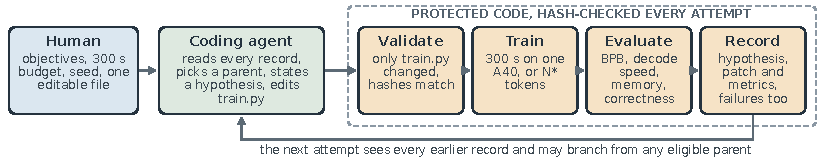
\includegraphics[width=\linewidth]{figures/research_loop_compact.pdf}
\caption{The AutoPareto loop. The agent proposes each attempt, and protected code (dashed box) validates, trains, measures and records it.}\label{fig:loop}
\end{figure}

\section{Related work}\label{app:related}
Operator-level, grammar-based and multi-objective architecture search \citep{primer,einspace,mote,monaq}, multi-fidelity allocation \citep{hyperband,bohb} and agentic research systems \citep{autodiscovery,mlestar,airesearcher,mledojo} are established, as are budget effects on model rankings \citep{dehghani2022efficiency,geiping2023cramming,hoffmann2022chinchilla}. The classical comparators are random search, TPE \citep{bergstra2011tpe}, MOTPE \citep{ozaki2020motpe}, NSGA-II \citep{deb2002nsga2} and CMA-ES \citep{hansen2001cmaes} over a fixed parameter vector, and \citet{ferreira} compare LLM agents with such optimizers on autoresearch. Primer searches compositions of low-level operations and finds stronger operator-level novelty than our numerical edits. Our architectural changes (fewer layers, smaller batches, attention windows) are not novel in themselves. Our contribution is an audit of what a resource contract rewards, with matched-exposure verification. The zero-shot suite is ARC-Easy \citep{clark2018arc}, PIQA \citep{bisk2020piqa}, LAMBADA \citep{paperno2016lambada} and BLiMP \citep{warstadt2020blimp}.

\section{Every search approach}\label{app:approaches}
\begin{table}[H]
\caption{Every search approach and what became of its recipes. Attempts: scheduled (completed and trained). Best val BPB: the lowest validation BPB of one archived 300\,s discovery run, per seed for AutoPareto (0 / 1 / 42) and for AutoResearch's 50-attempt campaign / 5-attempt follow-up. These are single noisy runs (pooled seed SD \CRPooledSD), comparable only within one seed and phase: the starting model's score differs by \CRBaseSeedEffect{} BPB between seeds 0 and 42, and the extended harness is another setting. Verified: retrained on new seeds in the seeds 3 to 5 panel (Table~\ref{tab:benchseeds}), E1, the Opus retraining or the 13-recipe test (Table~\ref{tab:verify}), or re-measured on a fresh A40.}\label{tab:approaches}
\centering\scriptsize\setlength{\tabcolsep}{3pt}% Generated by analysis/cr_v3.py (cr_stats.json archive_bests; cr_v2.json extended arms). Do not edit by hand.
\begin{tabular}{@{}>{\raggedright\arraybackslash}p{2.25cm}>{\raggedright\arraybackslash}p{2.9cm}>{\raggedright\arraybackslash}p{1.55cm}>{\raggedright\arraybackslash}p{1.55cm}>{\raggedright\arraybackslash}p{1.7cm}>{\raggedright\arraybackslash}p{2.95cm}@{}}
\toprule
Approach & What it changes & Phase, seed & Attempts (done) & Best val BPB & Verified recipes \\
\midrule
Random search & random samples from a fixed list of 15 settings & original, 42 & 25 (23) & 1.1038 & best-BPB recipe: 13-recipe test \\
TPE & model of which settings gave low BPB & original, 42 & 25 (23) & 1.0977 & best-BPB recipe: panel, 13-recipe test \\
MOTPE & TPE for BPB, speed and memory together & original, 42 & 25 (24) & 1.0981 & best-BPB recipe: panel, 13-recipe test \\
NSGA-II & evolving population, three objectives & original, 42 & 25 (23) & 1.1077 & best-BPB recipe: 13-recipe test \\
CMA-ES & adapted search distribution, BPB only & original, 42 & 25 (25) & 1.1083 & best-BPB recipe: 13-recipe test \\
AutoResearch & GPT-5.6 edits \texttt{train.py}, BPB only & original, 42 & 50 (19) + 5 (3) & 1.0968 / 1.0950 & AR-ref (exp 68): panel, E1, 13-recipe test \\
AutoPareto, GPT-5.6 & edits \texttt{train.py}, three objectives & original, 0 / 1 / 42 & 75 (74) & 1.0933 / 1.0958 / 1.0940 & GPT A22, GPT A25, GPT A24: panel, 13-recipe test; GPT A22: E1 \\
AutoPareto, GPT-5.6 & also edits inference code & extended, 3 & 22 (22) & 1.1016 & none (A14: campaign record) \\
AutoPareto, Opus 5.5 & also edits inference code & extended, 3 & 27 (25) & 1.0962 & A23, A24, A27: retrained, 13-recipe test \\
\bottomrule
\end{tabular}

\end{table}
The classical optimizers are Optuna samplers over one frozen space of 15 discrete settings of the original \texttt{train.py}: depth 6 to 10, three aspect ratios, two head sizes, four attention-window patterns, three key-value head ratios, total batch $2^{17}$ to $2^{19}$, four learning rates, weight decay, warm-up, warm-down, final learning-rate fraction and Muon Newton--Schulz steps. Random search, TPE and CMA-ES minimize validation BPB, while MOTPE and NSGA-II (population 8) optimize BPB, decode speed and memory together. They could not edit code, so their space excludes the smaller batches and shallower models the agents reached. All five ran 25 trials on seed 42 under the same 300\,s contract and evaluator family, and OOM failures counted as trials. Their seeds 0 and 1 were registered but never run. Only the best-BPB recipes of TPE and MOTPE entered the 201.3M-token panel.

\section{Who could edit the inference code}\label{app:access}
Every AutoPareto agent could write only \texttt{train.py}, and in every AutoPareto campaign that file could define \texttt{build\_inference\_adapter(model)}, a documented hook whose \texttt{prefill} and \texttt{decode\_one} the protected benchmark then timed in its own loop, with its own prompts, correctness checks and repetitions. The original program lists ``a candidate cache adapter that satisfies the protected interface'' as part of the research surface and the extended program ``an inference adapter compatible with the protected interface''. Both frame the adapter as needed when an architecture changes the cache layout, and neither mentions CUDA graphs, compilation, kernels or quantization. The starting \texttt{train.py} of both phases contained no generation code. Without an adapter, the protected benchmark ran its own re-implementation of the model, so architecture edits changed the timed computation and edits to the candidate's forward code did not. The 50-attempt AutoResearch campaign predates the hook.

\begin{table}[H]
\caption{The inference-editing surface and conditions of each AutoPareto search, read from the candidate sources and attempt records. ``Own inference code'' counts candidate sources that define the hook. Opus's failed A9 also wrote one, but its source was not kept. Opus's evaluator change fixed an FP32 correctness check that crashed on the first candidate adapter (A8), which was then re-run unchanged.}\label{tab:access}
\centering\scriptsize\setlength{\tabcolsep}{3pt}\renewcommand{\arraystretch}{1.12}% Generated by analysis/cr_r8.py from queue/autopareto-seed*/ and the extended attempt records. Do not edit by hand.
\begin{tabular}{@{}>{\raggedright\arraybackslash}p{3.0cm}>{\raggedright\arraybackslash}p{3.15cm}>{\raggedright\arraybackslash}p{3.15cm}>{\raggedright\arraybackslash}p{3.15cm}@{}}
\toprule
 & GPT-5.6, original (3 campaigns) & GPT-5.6, extended & Opus 5.5, extended \\
\midrule
Writable file & \texttt{train.py} & \texttt{train.py} & \texttt{train.py} \\
Own-inference hook & documented & documented & documented \\
Program; start (SHA-256) & \texttt{af42d041} then \texttt{7d6817f0}; \texttt{428e22f1}, \texttt{eb267bef} & \texttt{8acffb40}; \texttt{b2fb8788} & \texttt{8acffb40}; \texttt{b2fb8788} \\
Decode benchmark & 256 in, 256 out, 10 repetitions & 1{,}024 in, 128 out, bracketed & 1{,}024 in, 128 out, bracketed \\
Model, reasoning & \texttt{gpt-5.6-sol}, high & \texttt{gpt-5.6-sol}, high & \texttt{claude-opus-5-5}, xhigh \\
Execution & agent app, instruction-based isolation & container, shell inside & host, file tools only \\
Call timeout & none recorded & 600\,s & 600\,s then 900\,s (from A10) \\
Evaluator (SHA-256) & original runner & \texttt{f05d47a1} & \texttt{f05d47a1} then \texttt{c9b632e6} (A8~on) \\
Attempts (completed) & 75 (74) & 22 (22) & 27 (25) \\
Attempts defining their own inference code & 0 of 75 & 0 of 22 & 19 of 25 valid (first: A8) \\
\bottomrule
\end{tabular}

\end{table}

What differed was the search. In the original campaigns every edit sat in the hyperparameter block, the KV-head setting or optimizer plumbing, and the offered ``systems'' change category was never used. In the extended run GPT-5.6 changed architecture or optimization in all \CRCxAttempts{} attempts, mostly by one or two lines, and its hypotheses never mention an adapter, graph or compilation. Opus wrote its first adapter at A8, to cut memory, and announced graph replay as its next step. The original program also made inference work costly: a failed cache check counted as a dominated crash and paused the whole campaign. The extended arms differed in reasoning setting, isolation, call timeout, harness repairs and attempt count, and each ran once. We therefore report the difference as two observed search strategies under equal access, not as a property of either model. The audit with exact file and attempt citations is \path{audit/camera_ready_2026/26_INFERENCE_EDITING_AUDIT.md}.

\section{Reproducibility Statement}\label{app:repro}
\paragraph{Code and artifacts.} \releasepending The public artifact for this paper, to be released at \url{https://github.com/ramisworld/AutoPareto}, contains:
{\setlength{\leftmargini}{1.2em}\begin{itemize}\setlength{\itemsep}{0pt}\setlength{\parskip}{0pt}\setlength{\topsep}{2pt}
\item the frozen recipe sources and protocol manifests,
\item the per-experiment registry with hypotheses, patches, parents, decisions and failures,
\item the fixed-time confirmation and ablation records,
\item the per-run records of the 21-run panel and the 24 E1 runs, with the E1 plan and analysis,
\item the Opus retraining and ablation plans, run records (raw benchmark records archived), analysis and audit record,
\item the extended-experiment histories of both agents, including failures,
\item the Opus frontier re-verification and downstream records,
\item the 13-recipe test's pre-registration, plan, amendments A1 to A4 and incident log, with its training, inference and lm-eval run records and analysis,
\item the selection manifests (\texttt{autopareto\_confirmation\_selection.json}, SHA-256 prefix \texttt{72d58664}, and \texttt{autopareto\_primary\_confirmation\_plan.json}),
\item the analysis and audit scripts, and environment pins.
\end{itemize}}
Provider-side agent state, the dataset cache and large checkpoints remain private. Checkpoint hashes are published.

\paragraph{How to run it.}\label{app:howto} % Hand-written from paper/camera_ready/REPRODUCE.md. Every path and flag below was checked against the source
% (argparse) on 2026-11-14, and the 13-recipe (Phase 6) lines on 2026-11-18; no command was executed for this revision.
Full commands and their private dependencies are in \path{paper/camera_ready/REPRODUCE.md}. Nothing below was re-executed for this revision, and every flag shown exists in the script's argument parser.

\emph{Level 1, artifacts (no GPU).} Python 3.10 with the pins in \path{paper/requirements.txt} and Tectonic. The build recomputes every number, table and figure and stops if any value differs from the committed audit by more than $10^{-9}$. It needs the full evidence tree (database snapshot, campaign histories, selection manifests), which is part of the pending release. The pre-registered analyses rerun on a CPU from committed records.
\par\begingroup\footnotesize
\begin{verbatim}
AUTOPARETO_EVIDENCE_ROOT=<evidence tree> sh paper/build_camera_ready.sh
E1=results/camera_ready_2026/amendment1/E1
python3 scripts/analyze_camera_ready_e1.py --runs-root $E1 --output-dir <out>
python3 scripts/analyze_e1_exposure_decomposition.py \
    --runs-root $E1 --out-dir <out>
python3 scripts/analyze_phase5.py --out <out>
python3 analysis/cr_p6.py    # 13-recipe test, from its run records
\end{verbatim}
\par\endgroup

\emph{Level 2, recipes (one A40).} \path{prepare.py} downloads the ClimbMix shards and rebuilds the tokenizer, whose hashes are checked against \path{study/contracts_2026/provenance/tokenizer_manifest.json}. Each executor only validates unless \texttt{-{}-execute} is passed. Frozen sources: GPT A22 \path{results/candidates/autopareto-seed0-20260731/0022-train.py}, AR-ref \path{results/candidates/autoresearch-diagnostic5-seed42-20260724/0005-train.py}, Opus \path{evaluation/phase5a_sources/}; the 13-recipe plan \path{evaluation/phase6_unified_plan.json} lists all 13 by hash. Its 300\,s and lm-eval stages run under amendment A1 (\path{scripts/run_phase6_p2.py}), and amendments A2 to A4 have their own runners (\path{scripts/run_phase6_a2.py}, \texttt{\_a3}, \texttt{\_a4}). The shard revision and the flash-attention kernel are not pinned in code, the lockfile is not yet on a public branch, and the E1 executor refuses to write into an output root that already holds the committed E0 results.
\par\begingroup\footnotesize
\begin{verbatim}
python prepare.py --num-shards 10 --download-workers 8
python scripts/run_camera_ready_e0_e1.py --stage E0 --execute
python scripts/run_camera_ready_e0_e1.py --stage E1 --execute
python scripts/run_phase5a_opus_fixed_tokens.py --execute
python scripts/run_phase6.py --stage train --execute
python scripts/run_phase6.py --stage inference --block P0a --execute
python scripts/run_phase6_p2.py --stage fixed --execute
\end{verbatim}
\par\endgroup

\emph{Level 3, agent campaigns.} The controller of the extended experiments runs a campaign with Claude Code or Codex CLI. Its programs are in \path{study/contracts_2026/programs/}, the Claude command line and its permission checks in \path{study/contracts_2026/isolation.py}, and \path{study/contracts_2026/tools/dry_run_claude_campaign.py} rehearses a campaign offline with a fake CLI and a mocked GPU. The \texttt{run} subcommand also needs the state root, manifest, baseline record and GPU-host arguments listed in \path{REPRODUCE.md}. Pod setup is partly manual, the Codex container image was not preserved, and the original campaigns have no single entry point.
\par\begingroup\footnotesize
\begin{verbatim}
python3 -B -m study.contracts_2026.campaign_controller {dry-run,preflight,run} \
    --agent-backend {claude,codex} --model <id> --reasoning <effort> \
    --scientist-timeout-seconds 600 ...
\end{verbatim}
\par\endgroup


\paragraph{Model panel and sources.} Each recipe is identified by the SHA-256 of its exact \texttt{train.py} (panel manifest \path{evaluation/phase1_public_manifest.json}): baseline \texttt{428e22f1}, AR-ref \texttt{b3a961ee}, TPE \texttt{8547b278}, MOTPE \texttt{62882a20}, GPT A22 \texttt{55a7fd8b}, GPT A24 \texttt{6d0d8d1d} and GPT A25 \texttt{36e3ad91} (first four bytes). GPT A22 has 29,360,392 parameters at depth 4, width 512, 4 query and 4 key-value heads and window pattern SSSL; AR-ref has 50,332,176 parameters at depth 8, width 512, 4 and 4 heads and window pattern SSSS.

\paragraph{Data.} Training shards were read from the \texttt{main} branch of \texttt{karpathy/climbmix-400b-shuffle}. Their revision is not pinned in code. Only the held-out shard is pinned: \texttt{shard\_06541.parquet} at revision \texttt{915333b4f8b8684f39aeaafea600fea6f43fb703} (SHA-256 recorded per run), 2,560 segments and 5,242,880 evaluated tokens. Sequences are 2,048-token packed with a project tokenizer of 8,192 entries, hashed for the panel, E1 and the extended experiments (\texttt{tokenizer.pkl} \texttt{888c9fa8}) but rebuilt on each pod and unhashed during discovery. Downstream datasets are pinned by revision.

\humanauthor[P2-11]{\textbf{Data integrity.} The canonical validation value for panel runs is the panel results file. Database rows differ from it by at most $2.4\times10^{-5}$ and held-out values agree exactly. Held-out BPB exceeds validation BPB by \CRHeldValOffLo--\CRHeldValOffHi{} depending on the recipe, so recipes are compared only within one metric. Identical token streams across panel recipes were verified at run time, and E1's 24 runs and the Opus retraining's \CRMTRuns{} passed every pre-registered integrity gate on the first attempt.}

\paragraph{Training protocol.} Panel seeds are 3, 4 and 5. Each run processes exactly \CRPanelBudget{} counted tokens, and every optimizer update, including the first eleven, is counted training. The first eleven updates (1,441,792 tokens) are excluded only from the steady-state timing estimate. GPT A22, A24 and A25, AR-ref, TPE and MOTPE use total batch 131,072 with device batch 64 and no gradient accumulation (1,536 updates). The baseline uses total batch 524,288 with accumulation 4 (384 updates). Learning-rate and weight-decay progress is the fraction of the token budget consumed. The Muon \citep{jordan2024muon} momentum warm-up stays step-based (300 updates). Software per era is in Table~\ref{tab:env}.

\paragraph{E1.} Plan \path{evaluation/camera_ready_e0_e1_plan_amendment1.json} (SHA-256 \texttt{89f29015}, committed 2026-11-04) is amendment 1 of plan \texttt{806a6397}, written after the original E0 halted on one run's update count (666 against a window of 669--681 on an A40 about 1\% slower) and approved by the PI. It made that window diagnostic and re-ran E0 in full, leaving gates, tolerances, cells, seeds and analysis unchanged. It fixes the recipes, budgets (88,604,672, 157,286,400 and 201,326,592 tokens; 300\,s), seeds (6, 7, 8), integrity gates, retry policy, analysis script and decision rules. Held-out BPB is primary and validation BPB secondary. Its hypotheses: \emph{H-E1a}, $\Delta=\mathrm{BPB}(\text{GPT A22})-\mathrm{BPB}(\text{AR-ref})$ increases monotonically with training tokens; \emph{H-E1b}, $\Delta\le0$ at the discovery-scale budget (88.6M tokens, 676 updates). H1, that GPT A22's fixed-time lead reverses at matched tokens on new seeds, was formulated retrospectively after the original experiments. The executor requires a recorded E0 pass under the same plan hash. E1 ran on 2026-11-07 on one A40 (24 of 24 runs passed on the first attempt; \CREOneHours{} A40-hours). Deviation: the plan's hardware note names the A40 on which E0 passed, which was no longer available; E1 ran on another A40 with the same driver, where training throughput matched E0 (AR-ref \CREOneTputAR{} and GPT A22 \CREOneTputAP{} tokens/s across runs, against \CREZeroTputAR{} and \CREZeroTputAP{} at E0).

\paragraph{Opus retraining and inference ablations.} Plans \path{evaluation/phase5a_opus_fixed_tokens_plan.json} (SHA-256 \texttt{a47f81b7}) and \path{evaluation/phase5b_inference_ablation_plan.json} (\texttt{94727990}) and the prose pre-registration \path{evaluation/PHASE5_PREREG.md} were committed on 2026-11-08 before any run. The primary test is each recipe's $\Delta$ against AR-ref. An E1 extension registered on 2026-11-02 for the single Opus winner, at all four E1 cells including 300\,s, was not executable: its frozen adapter refuses all three Opus sources, whose training-loop driver Opus rewrote for the time contract, so it stays unrun. The new plan has no 300\,s cell, so the fixed-time Opus--AR-ref comparison is post hoc. The retraining used two scripted, gated changes. (i) A mapping restores the panel baseline's text for exactly the contract-T driver lines (progress call, clock, time stop, constants and prints) and moves the recipe's post-training storage lines before the final evaluation. Model and optimizer definitions stay byte-identical, and the unchanged protected transform then sets token-fraction learning-rate progress and the exact-token stop (Opus's own runs used time-fraction progress). (ii) An export applies each recipe's own post-training storage conversion (bf16 matrices; also int8 tables for A27) to the in-loop checkpoint with bit-exact load gates, so the evaluator scores the deployed model as in the extended experiments. An AR-ref drift control ran first (rule: within 0.005 BPB of E1; observed \CRMTDriftAbs), then seeds 6, 7 and 8 with a Latin square over recipes. All \CRMTRuns{} runs passed on the first attempt (\CRMTHours{} A40-hours with the downstream suite). The ablations replace only \texttt{build\_inference\_adapter} in the frozen sources and run the frozen protected benchmark (SHA-256 equal to the re-verification's) in candidate-only mode: each of 18 checkpoint--variant cells twice, forward then reversed, with the same-session baseline at the start, middle and end (\CRIARuns{} runs, \CRIAHours{} A40-hours, over the estimate but inside the pre-registered $2\times$ stop rule). Correctness passed in every run on the 64- and 256-token prefixes it checks, which do not reach the timed decode window after the 1{,}024-token prompt (\S\ref{sec:inference}). \CRIAUnstable{} graph-free runs failed the frozen stability rule and are reported as measured. Fusion also lengthens prefill (\CRThreePreNoFusion{} to \CRThreePreOpus{} ms), so its end-to-end gain is at most \CRIAFusionEtoEHi$\times$. Custom attention adds \CRIAAttnLo$\times$ to decode speed and the ring cache \CRIARingLo$\times$. A diagnostic \texttt{torch.profiler} census counted kernels and launches per decode token (32 tokens after 8 warm-up). End-to-end throughput in the ablations and Table~\ref{tab:agents} is the median over measured repetitions. The campaign records (Figure~\ref{fig:agents}b) store one generation per attempt. The recorded end-to-end rate equals 128 tokens divided by prefill plus 127 decode steps to within 1.5\% in every ablation cell, which is how Figure~\ref{fig:inference}b decomposes it.

\paragraph{The 13-recipe test.} Pre-registration \path{evaluation/PHASE6_PREREG.md} and plan \path{evaluation/phase6_unified_plan.json} (SHA-256 \texttt{dc1e605e}) were written on 2026-11-16 before any of its GPU measurements: no search and no agent calls, only the 13 frozen sources, retrained on seeds 6 to 8 for 201{,}326{,}592 tokens and for 300\,s and timed with one inference benchmark, all new runs and all timing on one A40 (driver 595.91.07); the reused runs below were trained on the A40s of E1 and the Opus retraining. Runs reused from E1 (AR-ref and GPT A22, both contracts) and the Opus retraining (Opus, 201.3M tokens) are hash-checked; drift controls on the new A40 reproduced AR-ref, GPT A22 and Opus A23 at 201.3M tokens within 0.0021 held-out BPB (rule: 0.005) and AR-ref at 300\,s within 0.0003. Opus's 300\,s runs use the mapped sources of the Opus retraining in E1's fixed-time cell. Four documented amendments changed execution, never measurement: A1 moved the 300\,s runs' data and run directories to local disk after network-storage stalls and added a timing-anomaly gate (3\,s of slow steps; every run passed, at most \CRSixFixedMaxExcess\,s), validated by a pilot, and fixed the lm-eval task list before any lm-eval run; A2 re-ran one matched-token run (MOTPE, seed 8) whose two attempts failed on a stale network file handle; A3 ran the frozen downstream stage with a database setting it omitted (taken from the Opus retraining's runner); and A4 restricted the lm-eval cross-check to ARC-Easy, PIQA and LAMBADA after a diagnostic traced BLiMP's 1-point gap to lm-eval's template (Table~\ref{tab:lmeval}). A host restart during the test (incident 5) changed the NVIDIA driver from 595.91.07 to 595.112.07 on the same GPU, so the 300\,s runs, MOTPE's seed-8 runs, the anchors and four Opus controls used the newer driver (Table~\ref{tab:env}). The AR-ref 300\,s drift control ran on it and still reproduced E1, and three anchors re-measured seed-6 recipes on it: their speed-ups changed by at most \CRSixAnchorSpeedMax\%, absolute decode rates by up to \CRSixAnchorDecodeMax\%, and Opus A23's prefill from \CRSixAnchorPreA{} to \CRSixAnchorPreB{} ms, which is why end-to-end gains vary between sessions. One run's training throughput (GPT A24, seed 6, matched tokens) is unreliable because of a storage stall; its quality is unaffected and no table uses it. Every incident, approval and amendment is logged with hashes in \path{evaluation/PHASE6_INCIDENTS.md}. Software: training PyTorch 2.9.1, inference PyTorch 2.8.0 (both CUDA 12.8), lm-evaluation-harness 0.4.13.

\par\medskip
\begin{table}[H]
\caption{Recorded software environment by era. Panel, Pair-A (extended experiments), E1, Opus-test and 13-recipe rows are read from their run records. Other rows are from the provenance audit. $^\dagger$Driver 595.112.07 after the host restart of 2026-11-16 (Appendix~\ref{app:repro}).}\label{tab:env}
\centering\scriptsize% Generated by analysis/cr_v2.py from table_env.tex (cr_tables.py) plus the E1 and Phase 5 records;: panel row from run_metadata.json/final_inference.json (21 runs); Pair-A row from the v2 manifest; other rows from audit REPRO section D.1. Do not edit by hand.
\begin{tabular}{p{2.1in}llll}
\toprule
Era & Python & PyTorch & CUDA & Driver \\
\midrule
Discovery and fixed-time re-runs (Jul 22--Aug 12) & 3.10 (from tracebacks) & not recorded & not recorded & not recorded \\
Inference canary, session 4 (Aug 16) & 3.12.3 & 2.8.0+cu128 & 12.8 & 570.195.03 \\
Matched-token panel, 21 runs (Aug 25--27) & 3.10.18 & 2.9.1+cu128 & 12.8 & 570.211.01 \\
Pair-A pilot (Sep 6--7) & 3.12 & 2.9.1+cu128 & 12.8 & not recorded \\
Pair-A Codex arm, continuation (Sep 16) & 3.12 & 2.8.0+cu128 & 12.8 & not recorded \\
Pair-A Opus 5.5 arm (Nov) & 3.12 & 2.8.0+cu128 & 12.8 & not recorded \\
E1 token sweep, 24 runs (Nov 7) & 3.10.18 & 2.9.1+cu128 & 12.8 & 595.91.07 \\
Opus retraining, 10 runs (Nov 8) & 3.10.18 & 2.9.1+cu128 & 12.8 & 595.91.07 \\
Inference ablations, 39 runs (Nov 8) & not recorded & 2.8.0+cu128 & 12.8 & 595.91.07 \\
13-recipe training, 61 runs (Nov 16--17) & 3.10.18 & 2.9.1+cu128 & 12.8 & 595.91.07$^\dagger$ \\
13-recipe inference, 61 runs (Nov 16--17) & 3.12.3 & 2.8.0+cu128 & 12.8 & 595.91.07$^\dagger$ \\
13-recipe lm-eval 0.4.13, 39 runs & 3.10.18 & 2.9.1+cu128 & 12.8 & not recorded \\
\bottomrule
\end{tabular}

\end{table}

\paragraph{Inference and memory protocol.} Every comparison of recipes on decode speed or memory uses one benchmark, protocol \texttt{autopareto\_search\_inference\_bracketed\_v2}: BF16, batch one, greedy decoding, 1,024 input and 128 generated tokens over 8 fixed prompts. After a 20\,s discarded warm-up it runs eight rounds of baseline, candidate and baseline windows, each at least 8\,s of cached decoding (127 transitions per generation). A candidate's decode rate is the median of its eight window rates; its speed-up is the median of the eight ratios of its window rate to the baseline rate interpolated from the windows just before and after it, so drift common to both cancels. Speed-ups divide by this bracketing registered baseline, the starting model of the extended campaigns; whole-generation gains divide by the Baseline recipe's own runs in the same test, the original starting model (both 8 layers, 50.3M parameters), and dividing Opus's decode rate by the Baseline recipe's instead gives \CRSixDecXVsBaseRecipe$\times$. Prefill and end-to-end speed are recorded but not scored. The 13-recipe test ran this protocol on every recipe in its own form (its own adapter where it defines one, otherwise the protected canonical adapter), after the correctness check below. Controls, as pre-registered: an uncached decode of every recipe; Opus's adapter with graph, compiled regions, split-key attention and ring cache all off; and the protected canonical adapter forced on Opus, which does not compute Opus's function (19 to 30 hard mismatches) and is therefore not timed. Peak memory is \texttt{torch.cuda.max\_memory\_allocated()} after \texttt{reset\_peak\_memory\_stats()}, with weights resident and reserved memory excluded.

\paragraph{Timing-stability flags.} The protocol marks a run unstable when its eight ratios vary too much: their interquartile range exceeds 2\% of their median, or their coefficient of variation exceeds 5\% (\path{study/contracts_2026/benchmark_policy.py}). \CRSixUnstableRuns{} of the 39 runs were flagged: \CRSixFlagDrift{} exceeded the 2\% limit and \CRSixFlagCVOnly{} (\CRSixFlagCVOnlyName) only the 5\% limit (\CRSixFlagCV{} exceeded the CV limit in all). A flag concerns timing stability, not correctness: every flagged run passed the correctness check. The protocol applies the same limits to each arm's windows as diagnostics. In all \CRSixFlagBaseDrift{} flagged runs at least one of the two baseline window sets varied by more than 2\% of its median, and in \CRSixFlagCandDrift{} the candidate's own windows did too, while in \CRSixCancelled{} unflagged runs the candidate's windows varied by more than 2\% but the ratios stayed within the limits, which is the drift the bracketing is designed to cancel. Opus's graph-replayed decoding varied by at most \CRSixOpusWinIQR\% across its windows, the recipes on the reference decoder by up to \CRSixRefWinIQR\%. Flags cluster in time: \CRSixBlockFlags{} of the \CRSixBlockRuns{} runs started between \CRSixBlockStart{} and \CRSixBlockEnd{} UTC on 16 November were flagged, against \CRSixRestFlags{} of the other \CRSixRestRuns. This pattern fits timing variation on the host rather than a property of the recipes. Plausible sources are CPU scheduling and kernel-launch overhead (the starting model launches \CRIAKernBase{} kernels per decoded token from the CPU), GPU clock variation, driver effects and other load on the shared host, but the records hold no clock, CPU-load or profiler traces for these windows, so we attribute the flags to none of them. Flagged runs are reported as measured, neither re-run nor dropped. They differ from their recipe's unflagged seeds by at most \CRSixUnstableMaxDev\%; seed-to-seed variation of a recipe's decode rate reaches \CRSixSeedCVMax\%, and the bracketing baseline ranged from \CRSixBracketLo{} to \CRSixBracketHi{} tok/s across runs. A post hoc check (\texttt{stability\_check} in \texttt{analysis/cr\_p6\_paper.py}) recomputes each recipe's mean decode rate from its unflagged runs only: no mean moves by more than \CRSixStableShiftMax\%, and the Pareto frontier of the seed means (Figure~\ref{fig:unifiedscatter}) is unchanged under both contracts; ranking by the scored speed-up instead changes only which of the three Opus recipes, \CRSixOpDecSpread\% apart in decode rate, are on it. Three anchor runs re-measured seed-6 recipes after the driver change (13-recipe test paragraph above): speed-ups moved by at most \CRSixAnchorSpeedMax\% and absolute rates by up to \CRSixAnchorDecodeMax\%. \emph{What this resolves:} Opus's \CRSixSpeedLo$\times$ to \CRSixSpeedHi$\times$ decode speed-up, seen in every run of all three recipes and in two earlier sessions, is far larger than any of these variations, whereas differences of under about 10\% between recipes on the reference decoder (for example TPE, MOTPE and Random Search, Table~\ref{tab:verify}) are not resolved.

\paragraph{Full-workload correctness.} Before timing, each recipe's timed decoder generated 128 tokens greedily for each of the 8 prompts (positions 1,024 to 1,151), and the recipe's own uncached \texttt{model.forward} was run once over prompt and generated tokens (teacher-forced, BF16 autocast; \path{scripts/phase6_unified_inference.py}). At each position the generated token either \emph{agrees} with the reference's argmax; is a \emph{near-tie}, a disagreement where the reference's top logit exceeds the generated token's by at most 0.25 (a bfloat16 rounding tie); or is a \emph{hard mismatch}, which fails the run and leaves it untimed. Across the 39 runs, \CRSixTokensAgree{} of \CRSixTokensChecked{} tokens agree (\CRSixAgreePct\%), \CRSixNearTies{} are near-ties (largest reference margin \CRSixNearTieMaxDeficit{} logits) and \CRSixHardMismatches{} are hard mismatches; the largest absolute logit difference is \CRSixMaxLogitErr. Because the reference is teacher-forced on the generated sequence, a near-tie cannot change later positions of the comparison. The tokens of the timed function equalled the checked tokens in all \CRSixTimedEqual{} runs. Each Opus recipe has two sliding-window layers with 256-token windows, whose keys and values sit in ring buffers sized to the window, so every checked position reads a cache that has already wrapped. The check establishes greedy-token agreement up to BF16 near-ties on this workload; it does not establish identical logits, other prompts or lengths, larger batches or sampled decoding.

\paragraph{Earlier inference measurements.} During search the original campaigns timed decode on another workload, a 256-token prompt and 256 generated tokens (\texttt{inference\_benchmark.py} in \texttt{cached\_decode} mode, 2 discarded warm-ups and 10 measured repetitions), and the seeds 3 to 5 panel re-timed its recipes on that workload with adaptive stabilization (\texttt{autopareto\_inference\_stabilized\_v2}). Those values guided search and selection, appear here only as search-record values (Figure~\ref{fig:tracks}), are superseded by the 13-recipe test and remain in the released records. The extended campaigns, the re-measurement of Opus's frontier and the ablations used the benchmark above. On the fresh-A40 re-measurement the raw repeat records give medians over three repeats of \CROpAbsTwentyThree, \CROpAbsTwentyFour{} and \CROpAbsTwentySeven{} tok/s for Opus A23, A24 and A27, with bracketing baseline rates of \CRPTwoBaseLo--\CRPTwoBaseHi{} tok/s. The ablation session measured \CRIAAbsLo--\CRIAAbsHi{} tok/s for the same recipes as submitted. Speed-ups are medians of window ratios, not ratios of these medians, and the registered baseline's calibration run decoded \CRAgBaseDecode{} tok/s. The three Opus recipes differ in absolute rate by \CROpAbsSpreadPct\%, so their speed-ups (\CROpDecodeLo$\times$ to \CROpDecodeHi$\times$) differ mainly through the baseline windows. In the extended experiments, \CROpUncertain{} of Opus's \CROpValid{} valid results and \CRCxUncertain{} of Codex's \CRCxValid{} were speed-uncertain. In the Opus arm this drift came from the baseline brackets on noisier hosts, not from the candidates. When Opus's frontier was re-measured, \CROpStableRepeats{} of \CROpRepeats{} repeats passed the drift rule. In the ablations \CRIAUnstable{} of \CRIARuns{} runs, all host-bound runs without the graph, failed the frozen stability rule and are reported, not re-run.

\paragraph{Agents and harness.} Extended experiments, Codex arm: Codex CLI 0.153.0, \texttt{gpt-5.6-sol}, reasoning high, 600-second call timeout, containerized headless execution. Opus arm: Claude Code 2.1.318, \texttt{claude-opus-5-5}, effort \texttt{xhigh}, file tools only, 900-second call timeout from attempt 10. Both: one writable file, per-arm histories, training seed 3, contract T at 300.000 protected seconds. Contract N at $N^\star$ counted tokens, the largest multiple of 524,288 not above the median of three baseline calibration runs: 88,604,672 in the first launches (calibration runs 88,604,672, 88,080,384 and 88,604,672; \path{runs/pair-a/provenance/final_pre_study_manifest_repaired_20260903.json}) and 85,458,944 after recalibration on a new A40 from 2026-09-09 (new-A40 baseline registration). The frozen first 25 Opus attempts (\CROpValidFrozen{} valid) give frontier \CROpFrontierFrozen{} and best BPB \CROpBestFrozen. All \CROpAttempts{} give \CROpFrontierExtended. Original experiments: \texttt{gpt-5.6-sol} at high reasoning effort through the Codex desktop app (core 0.145--0.146 alpha), except seed-42 attempts 1--5, proposed in Cursor's agent with the same model and setting while Codex usage was exhausted. After the seed-42 rollback, attempt 5 (exp 92) re-ran the original attempt-5 change unchanged on a new pod, operated from a Codex thread set to medium effort. It is a replay, not a new proposal. Per-attempt attribution from the author's session logs: \path{audit/camera_ready_2026/25_HISTORICAL_AGENT_PROVENANCE.md}. Isolation in the original experiments was instruction-based, with hash-checked protected files. The loop of \S\ref{sec:loop} is implemented by the runner functions \texttt{validate\_autopareto\_proposal} and \texttt{raw\_pareto\_rows} (original) and by \texttt{campaign\_controller.py} and \texttt{campaign.py} (extended).

\section{Full statistics and benchmarks}\label{app:panel}
\begin{table}[H]
\begin{minipage}[c]{.61\linewidth}\centering\scriptsize\setlength{\tabcolsep}{4pt}% Generated by analysis/cr_v3.py from cr_v2.json (E1 e1_analysis.json; Phase 5 phase5_analysis.json). Do not edit by hand.
\begin{tabular}{@{}llccc@{}}
\toprule
Recipe & Budget & Tokens (M) & $\Delta$ held-out BPB [95\% CI] & Better \\
\midrule
GPT A22 & 300\,s & 88 / 158 & $-$0.002 [$-$0.020, +0.016] & 1/3 \\
GPT A22 & 88.6M tok. & equal & +0.038 [+0.022, +0.055] & 0/3 \\
GPT A22 & 157.3M tok. & equal & +0.040 [+0.023, +0.056] & 0/3 \\
GPT A22 & 201.3M tok. & equal & +0.042 [+0.029, +0.054] & 0/3 \\
\midrule
Opus A23 & 201.3M tok. & equal & +0.059 [+0.051, +0.066] & 0/3 \\
Opus A24 & 201.3M tok. & equal & +0.061 [+0.052, +0.070] & 0/3 \\
Opus A27 & 201.3M tok. & equal & +0.059 [+0.053, +0.064] & 0/3 \\
\bottomrule
\end{tabular}
\end{minipage}\hfill
\begin{minipage}[c]{.37\linewidth}\captionof{table}{Held-out BPB of each recipe minus AR-ref, paired by seed (seeds 6 to 8, 95\% $t$ intervals). Negative values favour the recipe. Better: seeds, out of three, in which the recipe beat AR-ref. Tokens: AR-ref / recipe. All rows pre-registered. Full statistics: Table~\ref{tab:e1full}.}\label{tab:results}\end{minipage}
\end{table}
\begin{table}[H]
\caption{Full statistics: recipe minus AR-ref in BPB (negative: recipe better), paired by seed, 95\% $t$ intervals (2 df). Tokens: AR-ref / recipe. E1 and Opus rows are pre-registered (E1's seeds and AR-ref runs). Seeds 0--2: the original fixed-time re-runs, validation only. Panel: the submitted version's 201.3M-token test (seeds 3--5). Better: seeds with $\Delta<0$ on the bold metric.}\label{tab:e1full}
\centering\scriptsize\setlength{\tabcolsep}{2.8pt}% Generated by analysis/cr_v2.py (E1 e1_analysis.json; cr_stats.json; Phase 5 phase5_analysis.json). Do not edit by hand.
\begin{tabular}{lllcllc}
\toprule
Recipe & Contract & Seeds & Tokens (M) & $\Delta$ held-out [95\% CI] & $\Delta$ validation [95\% CI] & Better \\
\midrule
GPT A22 & 300\,s, re-runs & 0--2 & 88.5 / 156.9 & n/a & \textbf{$-$0.0067} [$-$0.0130, $-$0.0003] & 3/3 \\
GPT A22 & 300\,s (E1) & 6--8 & 88.0 / 158.1 & \textbf{$-$0.0022} [$-$0.0205, +0.0160] & $-$0.0044 [$-$0.0124, +0.0036] & 1/3 \\
\midrule
GPT A22 & 88.6M tok. (E1) & 6--8 & 88.6 / 88.6 & \textbf{+0.0385} [+0.0222, +0.0547] & +0.0418 [+0.0343, +0.0493] & 0/3 \\
GPT A22 & 157.3M tok. (E1) & 6--8 & 157.3 / 157.3 & \textbf{+0.0396} [+0.0226, +0.0565] & +0.0430 [+0.0341, +0.0519] & 0/3 \\
GPT A22 & 201.3M tok. (E1) & 6--8 & 201.3 / 201.3 & \textbf{+0.0415} [+0.0287, +0.0544] & +0.0445 [+0.0364, +0.0527] & 0/3 \\
GPT A22 & 201.3M tok. (panel) & 3--5 & 201.3 / 201.3 & \textbf{+0.0420} [+0.0297, +0.0544] & +0.0451 [+0.0415, +0.0486] & 0/3 \\
\midrule
Opus A23 & 201.3M tok. & 6--8 & 201.3 / 201.3 & \textbf{+0.0587} [+0.0514, +0.0660] & +0.0620 [+0.0585, +0.0655] & 0/3 \\
Opus A24 & 201.3M tok. & 6--8 & 201.3 / 201.3 & \textbf{+0.0608} [+0.0516, +0.0701] & +0.0648 [+0.0620, +0.0677] & 0/3 \\
Opus A27 & 201.3M tok. & 6--8 & 201.3 / 201.3 & \textbf{+0.0586} [+0.0527, +0.0644] & +0.0620 [+0.0589, +0.0651] & 0/3 \\
\bottomrule
\end{tabular}

\end{table}

\begin{table}[h]
\caption{The 13-recipe test (Figure~\ref{fig:overview}): all 13 recipes, seeds 6 to 8 (means; held-out BPB $\pm$ seed SD). Inference: tokens/s and peak MiB, 1{,}024 input and 128 generated tokens, batch one. Accuracy after 201.3M tokens; GPT A24's ARC-Easy lead over AR-ref (+\CRSixArcBestOverAR{} points) exceeds the seed SDs, but no task leader's margin over the runner-up (at most \CRSixLeadRunnerMax) does. Bold: best; $^\star$: on the frontier of held-out BPB and decode speed in every seed under that budget (the stars of Figure~\ref{fig:overview}).}\label{tab:verify}\label{tab:bench}
\centering{\scriptsize\setlength{\tabcolsep}{3.0pt}\begin{tabular}{@{}lrrrrrrrrrr@{}}
\toprule
& & \multicolumn{2}{c}{Held-out BPB} & \multicolumn{3}{c}{Inference (1,024 in, 128 out)} & \multicolumn{4}{c}{Zero-shot accuracy (\%)} \\
\cmidrule(lr){3-4}\cmidrule(lr){5-7}\cmidrule(l){8-11}
Recipe & Params & 201.3M tok. & 300\,s & Decode & End to end & MiB & ARC-E & PIQA & LAMB. & BLiMP \\
\midrule
Baseline & 50.3M & 1.144{\tiny$\pm$0.005} & 1.240{\tiny$\pm$0.002} & 145 & 146 & 337 & 35.9 & 57.0 & 20.8 & 71.3 \\
\addlinespace[1.5pt]
AR-ref & 50.3M & \textbf{1.099{\tiny$\pm$0.004}}$^\star$ & 1.157{\tiny$\pm$0.004} & 145 & 145 & 337 & 36.2 & 58.1 & 21.9 & \textbf{74.5} \\
\addlinespace[1.5pt]
Random Search & 32.0M & 1.122{\tiny$\pm$0.001} & 1.158{\tiny$\pm$0.001} & 180 & 181 & 260 & 36.3 & \textbf{59.1} & 19.3 & 72.8 \\
TPE & 39.8M & 1.121{\tiny$\pm$0.001}$^\star$ & 1.156{\tiny$\pm$0.002} & 193 & 194 & 289 & 35.4 & 56.6 & 21.0 & 74.2 \\
MOTPE & 26.3M & 1.149{\tiny$\pm$0.006} & 1.165{\tiny$\pm$0.004} & 192 & 193 & 226 & 35.5 & 57.9 & 21.2 & 72.3 \\
NSGA-II & 50.3M & 1.114{\tiny$\pm$0.001} & 1.171{\tiny$\pm$0.001} & 148 & 149 & 337 & 35.5 & 57.3 & 20.9 & 74.4 \\
CMA-ES & 21.5M & 1.142{\tiny$\pm$0.001} & 1.164{\tiny$\pm$0.002} & 157 & 158 & 210 & 35.3 & 56.9 & 18.2 & 72.6 \\
\addlinespace[1.5pt]
GPT A22 & 29.4M & 1.141{\tiny$\pm$0.004}$^\star$ & \textbf{1.155{\tiny$\pm$0.004}} & 266 & 267 & 243 & 36.7 & 57.5 & 21.3 & 72.6 \\
GPT A24 & 17.9M & 1.187{\tiny$\pm$0.002} & 1.186{\tiny$\pm$0.001} & 364 & 366 & 183 & \textbf{38.1} & 58.5 & 19.7 & 68.7 \\
GPT A25 & 26.2M & 1.160{\tiny$\pm$0.006} & 1.163{\tiny$\pm$0.005} & 373 & 372 & 221 & 35.8 & 57.3 & 19.8 & 71.0 \\
\addlinespace[1.5pt]
Opus A23 & 26.2M & 1.158{\tiny$\pm$0.002} & 1.159{\tiny$\pm$0.003} & 4,579 & \textbf{672} & 110 & 36.5 & 58.4 & 21.7 & 71.1 \\
Opus A24 & 22.0M & 1.160{\tiny$\pm$0.001}$^\star$ & 1.160{\tiny$\pm$0.004}$^\star$ & \textbf{4,591} & 663 & 105 & 35.4 & 57.1 & 20.8 & 70.9 \\
Opus A27 & 26.2M & 1.158{\tiny$\pm$0.002}$^\star$ & 1.159{\tiny$\pm$0.002} & 4,583 & 664 & \textbf{96} & 36.7 & 57.9 & \textbf{22.3} & 70.7 \\
\bottomrule
\end{tabular}
}
\end{table}
\begin{table}[h]
\caption{The 13-recipe test: held-out BPB of each recipe minus AR-ref, paired by seed (seeds 6 to 8), with 95\% $t$ intervals (2 df). Positive: worse than AR-ref. Bold: interval excludes zero (per comparison, not adjusted for the 12 comparisons). Post hoc, with a Bonferroni adjustment ($t=\CRSixBonfT$, 2 df) \CRSixBonfTok{} of the 12 matched-token gaps stay resolved (not \CRSixBonfTokLost, each still worse in all three seeds; GPT A22's gap is also E1's single pre-registered comparison) and at 300\,s only \CRSixBonfTimeKept's. Seeds worse: seeds, of three, in which the recipe was worse.}\label{tab:paired6}
\centering\scriptsize\setlength{\tabcolsep}{4pt}\begin{tabular}{@{}lrrrr@{}}
\toprule
Recipe & 201.3M tokens & Seeds worse & 300\,s & Seeds worse \\
\midrule
Baseline & \textbf{+0.045 [+0.037, +0.053]} & 3 of 3 & \textbf{+0.083 [+0.078, +0.089]} & 3 of 3 \\
Random Search & \textbf{+0.023 [+0.009, +0.036]} & 3 of 3 & +0.001 [$-$0.007, +0.009] & 2 of 3 \\
TPE & \textbf{+0.021 [+0.010, +0.032]} & 3 of 3 & $-$0.001 [$-$0.011, +0.010] & 2 of 3 \\
MOTPE & \textbf{+0.050 [+0.043, +0.056]} & 3 of 3 & \textbf{+0.008 [+0.004, +0.012]} & 3 of 3 \\
NSGA-II & \textbf{+0.014 [+0.004, +0.025]} & 3 of 3 & \textbf{+0.014 [+0.005, +0.022]} & 3 of 3 \\
CMA-ES & \textbf{+0.043 [+0.035, +0.051]} & 3 of 3 & +0.007 [$-$0.006, +0.021] & 3 of 3 \\
GPT A22 & \textbf{+0.042 [+0.029, +0.054]} & 3 of 3 & $-$0.002 [$-$0.020, +0.016] & 2 of 3 \\
GPT A24 & \textbf{+0.088 [+0.077, +0.098]} & 3 of 3 & \textbf{+0.029 [+0.017, +0.041]} & 3 of 3 \\
GPT A25 & \textbf{+0.061 [+0.044, +0.077]} & 3 of 3 & +0.007 [$-$0.010, +0.023] & 2 of 3 \\
Opus A23 & \textbf{+0.059 [+0.051, +0.066]} & 3 of 3 & +0.002 [$-$0.002, +0.006] & 3 of 3 \\
Opus A24 & \textbf{+0.061 [+0.052, +0.070]} & 3 of 3 & +0.003 [$-$0.011, +0.017] & 2 of 3 \\
Opus A27 & \textbf{+0.059 [+0.053, +0.064]} & 3 of 3 & +0.002 [$-$0.004, +0.008] & 2 of 3 \\
\bottomrule
\end{tabular}

\end{table}
\begin{figure}[H]
\centering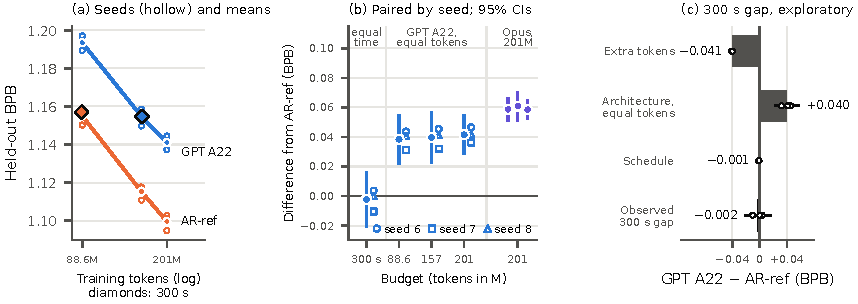
\includegraphics[width=\linewidth]{figures/cr_e1_full.pdf}
\caption{E1 in full (held-out BPB, seeds 6 to 8). (a) Every run: equal tokens (lines) and 300\,s (diamonds), where GPT A22 trains on \CREOneTokAP M tokens and AR-ref on \CREOneTokAR M. (b) Difference from AR-ref, paired by seed (95\% $t$ intervals): not resolved at equal time; GPT A22 worse for every seed at every token budget, and Opus's recipes worse still at 201.3M tokens. (c) Exploratory split of the 300\,s gap (means, 95\% intervals, seeds): GPT A22's extra tokens are worth about as much as its smaller architecture costs at equal tokens. The split was specified after the plan, before E1 results.}\label{fig:e1}\label{fig:e1split}
\end{figure}
\begin{table}[H]
\caption{Per-seed values of the earlier verification (the 13-recipe test's per-seed values are in the released data): held-out BPB and zero-shot accuracy in \% (LAMBADA: exact final word) after 201.3M training tokens, listed in seed order. The panel used seeds 3 to 5; E1 and the Opus retraining used seeds 6 to 8, so AR-ref and GPT A22 appear twice. An accuracy cell's seed SD is typically \CRNineBenchSDMed{} points (at most \CRNineBenchSDMax), so ARC-Easy, PIQA and LAMBADA barely separate recipes, while BLiMP tracks held-out BPB (panel $r=\CRCorrBLiMPHeld$). Chance is about 25\% on ARC-Easy and 50\% on PIQA and BLiMP. The extended GPT-5.6 campaign's recipes were not retrained at matched tokens.}\label{tab:benchseeds}
\centering\scriptsize\setlength{\tabcolsep}{3pt}% Generated by analysis/cr_r9.py (bench_data). Do not edit by hand.
\begin{tabular}{@{}llccccc@{}}
\toprule
Candidate & Seeds & Held-out BPB & ARC-Easy & PIQA & LAMBADA & BLiMP \\
\midrule
Baseline & 3, 4, 5 & 1.1431 / 1.1519 / 1.1448 & 36.0 / 33.6 / 36.3 & 56.9 / 57.7 / 57.5 & 20.1 / 20.1 / 21.2 & 72.3 / 71.2 / 70.6 \\
AR-ref & 3, 4, 5 & 1.1009 / 1.1009 / 1.0976 & 35.8 / 38.1 / 35.6 & 57.5 / 60.2 / 58.3 & 19.4 / 21.2 / 20.6 & 74.6 / 73.9 / 75.1 \\
TPE & 3, 4, 5 & 1.1145 / 1.1224 / 1.1213 & 36.7 / 34.7 / 35.6 & 58.4 / 57.6 / 57.0 & 22.8 / 21.0 / 20.4 & 74.1 / 72.6 / 73.2 \\
MOTPE & 3, 4, 5 & 1.1508 / 1.1491 / 1.1448 & 35.1 / 37.4 / 33.8 & 57.1 / 57.9 / 57.3 & 23.0 / 22.6 / 18.9 & 71.9 / 72.6 / 72.9 \\
GPT A22 & 3, 4, 5 & 1.1396 / 1.1487 / 1.1372 & 37.1 / 36.5 / 37.1 & 58.0 / 58.5 / 58.4 & 23.2 / 21.7 / 19.6 & 71.6 / 72.0 / 72.4 \\
GPT A24 & 3, 4, 5 & 1.1909 / 1.1917 / 1.1876 & 35.1 / 33.8 / 35.5 & 56.8 / 56.7 / 57.2 & 19.7 / 20.6 / 19.5 & 70.5 / 69.1 / 68.4 \\
GPT A25 & 3, 4, 5 & 1.1594 / 1.1589 / 1.1596 & 33.9 / 36.6 / 36.6 & 57.2 / 56.6 / 58.1 & 20.7 / 21.0 / 20.6 & 70.1 / 71.3 / 70.1 \\
\midrule
AR-ref & 6, 7, 8 & 1.0947 / 1.1010 / 1.1027 & 35.1 / 36.9 / 36.5 & 58.4 / 58.1 / 57.8 & 21.4 / 22.1 / 22.0 & 74.2 / 74.4 / 74.9 \\
GPT A22 & 6, 7, 8 & 1.1413 / 1.1372 / 1.1445 & 36.4 / 36.2 / 37.5 & 57.0 / 57.6 / 58.1 & 21.9 / 21.5 / 20.6 & 72.5 / 73.4 / 72.0 \\
Opus A23 & 6, 7, 8 & 1.1560 / 1.1604 / 1.1583 & 36.3 / 37.2 / 36.1 & 59.0 / 58.5 / 57.8 & 21.4 / 21.3 / 22.2 & 70.8 / 71.1 / 71.4 \\
Opus A24 & 6, 7, 8 & 1.1595 / 1.1616 / 1.1600 & 36.5 / 35.3 / 34.5 & 56.3 / 57.7 / 57.4 & 20.9 / 21.1 / 20.5 & 71.0 / 70.6 / 71.0 \\
Opus A27 & 6, 7, 8 & 1.1558 / 1.1594 / 1.1590 & 36.1 / 37.8 / 36.3 & 57.6 / 58.1 / 58.1 & 22.0 / 21.6 / 23.3 & 71.2 / 70.4 / 70.5 \\
\bottomrule
\end{tabular}

\end{table}

\begin{table}[H]
\caption{Further zero-shot tasks (lm-evaluation-harness 0.4.13) for all 13 recipes after 201.3M tokens: accuracy in \%, seed means over seeds 6 to 8 (seed SDs up to \CRSixLmSDMax{} points); WikiText: word perplexity, lower is better. Bold: best. At this scale ARC-Challenge, HellaSwag, OpenBookQA, WinoGrande and BoolQ sit near or below chance (25\%, 25\%, 25\%, 50\%; BoolQ's majority class is about 62\%), and their recipe ranking is unrelated to held-out BPB (Spearman $|\rho|\le\CRSixRhoNearMax$). WikiText perplexity ranks the recipes like held-out BPB ($\rho=\CRSixRhoWiki$), as BLiMP does in Table~\ref{tab:verify} ($\rho=\CRSixRhoBlimp$). A cross-check on three checkpoints reproduced the frozen evaluator's ARC-Easy, PIQA and LAMBADA exactly; lm-eval's BLiMP template scores each sentence with a leading space and reads about 1 point higher, so Table~\ref{tab:verify} keeps the frozen BLiMP (amendment A4).}\label{tab:lmeval}
\centering\scriptsize\setlength{\tabcolsep}{4pt}\IfFileExists{generated/camera_ready/table_unified_lmeval.tex}{\begin{tabular}{@{}lrrrrrrr@{}}
\toprule
Recipe & ARC-C & HellaSwag & WinoGr. & OBQA & SciQ & BoolQ & WikiText ppl \\
\midrule
Baseline & 19.3 & 27.1 & 49.5 & 13.3 & 71.5 & 53.8 & 128.6 \\
AR-ref & 19.2 & \textbf{27.5} & 51.1 & \textbf{15.5} & 72.3 & \textbf{58.7} & \textbf{106.2} \\
Random Search & 18.9 & 27.0 & 50.0 & 15.3 & 69.5 & 54.3 & 119.8 \\
TPE & 19.1 & 27.3 & 49.8 & 15.3 & 71.6 & 52.5 & 115.9 \\
MOTPE & \textbf{19.7} & 27.2 & 50.9 & 13.7 & 68.8 & 48.7 & 127.9 \\
NSGA-II & 19.0 & \textbf{27.5} & 51.7 & \textbf{15.5} & 71.0 & 57.6 & 109.1 \\
CMA-ES & 18.6 & 27.0 & 50.4 & 15.0 & 67.7 & 47.6 & 129.9 \\
GPT A22 & 19.2 & 27.4 & \textbf{52.0} & 14.6 & \textbf{73.6} & 46.2 & 125.0 \\
GPT A24 & 18.8 & 27.2 & 50.5 & 15.3 & 67.7 & 43.2 & 151.4 \\
GPT A25 & 18.3 & 27.3 & 51.5 & 14.2 & 69.0 & 53.8 & 135.2 \\
Opus A23 & 19.0 & \textbf{27.5} & 50.3 & 14.6 & 70.8 & 50.2 & 134.8 \\
Opus A24 & 18.9 & \textbf{27.5} & 49.8 & 15.4 & 70.4 & 56.3 & 136.0 \\
Opus A27 & 19.5 & 27.3 & 51.4 & 13.8 & 71.2 & 51.1 & 134.7 \\
\bottomrule
\end{tabular}
}{\authortodo{lm-eval table pending}}
\end{table}
\begin{table}[H]
\caption{\humancaption{P2-08}Selection funnel from discovery to the reported recipes, in time order. Step 2's rule was fixed before the first AutoPareto attempt. Steps 3 and 4 were chosen after the agents' scores, and for step 4 the seeds 0--2 re-runs, were known. Step 5 was pre-registered. Counts and dates: Appendix Table~\ref{tab:funnelfull}.}\label{tab:funnel}
\centering\scriptsize\setlength{\tabcolsep}{3pt}% Generated by analysis/cr_v3.py; facts asserted against table_funnel.tex (cr_tables.py). Do not edit by hand.
\begin{tabular}{@{}>{\raggedright\arraybackslash}p{4.3cm}l>{\raggedright\arraybackslash}p{6.4cm}@{}}
\toprule
Stage (2026) & Selection & What was kept \\
\midrule
1. Discovery (Jul 22--Aug 7) & agents & 75 AutoPareto attempts on seeds 0, 1 and 42 (plus AutoResearch, TPE, MOTPE) \\
2. Representatives (rule fixed Jul 27, \emph{before} discovery) & pre-specified & 11 AutoPareto recipes, including exp 109 (seed 42) \\
3. Four roles (Aug 10, \emph{after} discovery) & post hoc & 4 seed-0 recipes: exp 124, 134 (GPT A22), 136, 137; then seeds 0--2 re-runs \\
4. 201M-token panel (Aug 21--25, after step-3 re-runs) & post hoc & 3 of the 4 (exp 124 dropped, no rule recorded) + AR-ref, TPE, MOTPE, baseline \\
5. E1 and Opus retraining (Nov 4 and Nov 8) & pre-registered & GPT A22, AR-ref; Opus A23, A24, A27 (its whole frontier) \\
\bottomrule
\end{tabular}

\end{table}
\begin{table}[H]
\caption{Selection funnel with per-comparator counts (dates 2026), as recorded in the selection manifests.}\label{tab:funnelfull}
\centering\scriptsize\setlength{\tabcolsep}{3pt}% Generated by analysis/cr_tables.py (SNAPDB counts; selection manifest sha256 72d5866426b3aadf; plan sha256 08f123ea565ebae5; P1JSON). Do not edit by hand.
\begin{tabular}{p{1.42in}p{1.78in}p{0.88in}p{0.82in}}
\toprule
Stage & AutoPareto & AutoResearch & TPE / MOTPE \\
\midrule
Discovery attempts (Jul 22--Aug 7) & 75 (seeds 0, 1, 42) & 50\,+\,5 (seed 42) & 25\,+\,25 (seed 42) \\
Per-campaign representatives (rule fixed Jul 27; output Aug 5) & 11: exp 103, 108, 109, 124, 134, 136, 137, 147, 152, 158, 162 & exp 65, 68 & -- \\
Global four-role selector (Aug 10, after discovery) & 4, all seed 0: exp 124, 134, 136, 137 & 68 (65 incompatible) & best BPB: 183, 234 \\
201M-token panel (set Aug 21--25; run Aug 25--27) & 3: exp 134, 136, 137 (exp 124 dropped; no rule recorded) & 68 & 183, 234 \\
\bottomrule
\end{tabular}

\end{table}

\section{Extended agent experiments (Pair-A)}\label{app:agents}
\begin{table}[H]
\caption{Two agents under the identical fixed-time contract (extended experiments, seed 3). Opus rows: its frontier re-measured on a fresh A40 (protected BPB identical; medians of three repeats; end to end: median over repetitions of a 1{,}024+128-token generation against the baseline recipe's \CRAgEtoERefRep{} tok/s; a separate session from the 13-recipe test, whose whole-generation gain is \CRSixEtoEXLo$\times$, \S\ref{sec:inference}). Codex row: campaign record (stopped after \CRCxAttempts{} of 25 scheduled attempts). Baseline row: the registration calibration run.}\label{tab:agents}
\centering\scriptsize\setlength{\tabcolsep}{3.2pt}% Generated by analysis/cr_v2.py (Pair-A T-arm histories; Phase 2 re-verification). Do not edit by hand.
\begin{tabular}{lcccrccr}
\toprule
 & Valid / & Val BPB & Tokens & Params & \multicolumn{2}{c}{Speed-up vs baseline} & Peak \\
\cmidrule(lr){6-7}
Agent, attempt & attempts & $\downarrow$ & in 300\,s (M) & (M) & decode only & end to end & MiB \\
\midrule
Registered baseline (calibration run) & n/a & 1.1999 & 85.5 & 50.3 & 1.00 & 1.00 & 337 \\
Codex, best (A14) & 22/22 & 1.1016 & 126.6 & 24.6 & 1.32 & 1.32 & 239 \\
Opus 5.5, A23 & 25/27 & 1.0962 & 197.1 & 26.2 & 31.8 & 5.3 & 113 \\
Opus 5.5, A24 &  & 1.0995 & 198.4 & 22.0 & 30.9 & 5.3 & 97 \\
Opus 5.5, A27 &  & 1.0962 & 198.0 & 26.2 & 31.5 & 5.2 & 99 \\
\bottomrule
\end{tabular}

\end{table}
\begin{figure}[H]
\centering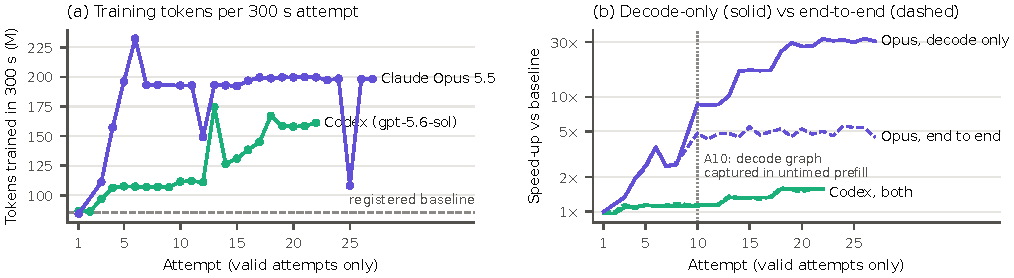
\includegraphics[width=.9\linewidth]{figures/cr_agents.pdf}
\caption{GPT-5.6 (Codex) and Claude Opus 5.5 under the same contract (valid attempts, at their attempt numbers). (a) Tokens trained in each 300\,s attempt. The registered baseline trained \CRAgBaseTok M. (b) Speed-up over the baseline from campaign records: decode-only (solid, scored) and end-to-end (dashed, recorded but not scored). The dotted line marks Opus A10, its first CUDA graph replay: the graph is recorded inside the untimed prefill, so decode-only speed jumps from \CREightOpSevenX$\times$ (A7) to \CREightOpTenX$\times$ while end-to-end speed rises far less. GPT-5.6 wrote no inference code, so its two curves coincide.}\label{fig:agents}
\end{figure}
\begin{figure}[H]
\centering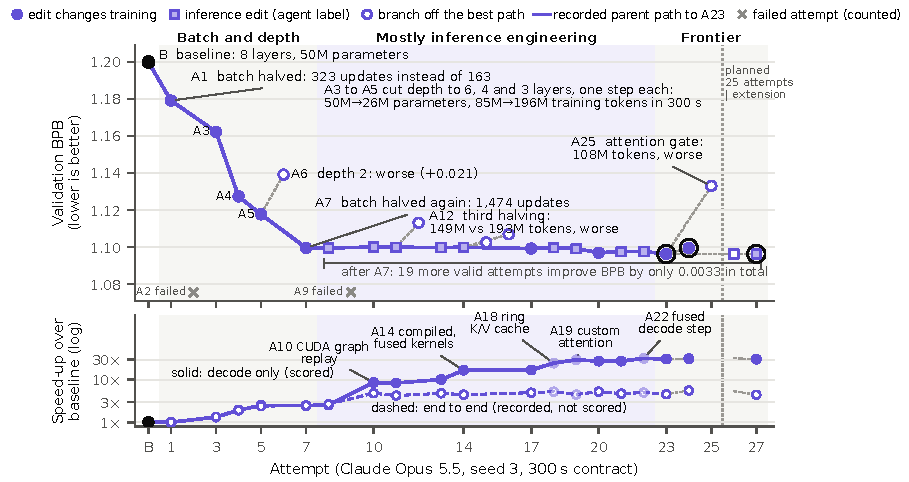
\includegraphics[width=\linewidth]{figures/cr_opus_lineage.pdf}
\caption{Complete lineage of the Opus campaign (extended experiments, seed 3, 300\,s), the full version of Figure~\ref{fig:opus}. Top: validation BPB of every attempt. Lines are recorded parent links, so every branch is real. Squares are attempts the agent labelled as inference edits, rings mark the final frontier (A23, A24, A27), and crosses are the two failed attempts, which still count. Bottom: speed over the baseline on the path to the best recipe, decode only (filled, scored) and end to end (hollow, not scored). Faded points are speed-uncertain.}\label{fig:opusfull}
\end{figure}
\begin{table}[H]
\caption{\humancaption{P2-15b}The fixed-time versus fixed-token pilot, read from every Codex launch (\texttt{gpt-5.6-sol}, seed 3, both arms from the same starting model: 8 layers, batch $2^{19}$ tokens, 50.3M parameters). Valid: completed and trained. Six fixed-time attempts of the 6 September warm-up launch checkpointed an untrained model because of a harness defect (\S\ref{sec:pilot}) and are excluded. Batch sizes, depths and parameters are read from each valid attempt's frozen source and record. Best: parameters of the attempt with the lowest validation BPB in that arm. Each launch ran each arm once, and the harness changed between launches.}\label{tab:pilot}
\centering\scriptsize\setlength{\tabcolsep}{4pt}% Generated by analysis/cr_v3.py from the Pair-A launch histories (read-only). Do not edit by hand.
\begin{tabular}{@{}llrlllr@{}}
\toprule
Launch & Arm & Valid / all & Batch sizes & Depths & Parameters (M), valid & Best: params \\
\midrule
Sep 5 & time & 0 / 2 &  &  &  &  \\
 & tokens & 1 / 2 & $2^{17}$ & 8 & 50.3 & 50.3 \\
\addlinespace[1pt]
Sep 6 (fresh) & time & 1 / 2 & $2^{18}$ & 8 & 50.3 & 50.3 \\
 & tokens & 2 / 2 & $2^{17}$, $2^{16}$ & 8 & 50.3 & 50.3 \\
\addlinespace[1pt]
Sep 6 (warm-up v2) & time & 2 / 8 & $2^{18}$, $2^{17}$ & 8 & 50.3 & 50.3 \\
 & tokens & 8 / 8 & $2^{19}$, $2^{18}$, $2^{17}$ & 10--12 & 64.9--135.3 & 85.9 \\
\addlinespace[1pt]
Sep 9 & time & 7 / 7 & $2^{19}$ & 7--8 & 16.3--39.8 & 16.3 \\
 & tokens & 7 / 7 & $2^{19}$, $2^{18}$ & 7--8 & 27.0--39.8 & 35.7 \\
\addlinespace[1pt]
Sep 14 & time & 22 / 22 & $2^{19}$, $2^{18}$, $2^{17}$ & 5--8 & 15.0--39.8 & 24.6 \\
 & tokens & 20 / 22 & $2^{19}$ & 6--8 & 33.6--47.2 & 47.2 \\
\bottomrule
\end{tabular}

\end{table}

\section{Agent reasoning under the time contract}\label{app:reasoning}
\begin{table}[H]
\caption{What the agents wrote before each attempt, next to what the attempt measured. Excerpts are verbatim from the attempt records (hypothesis, intended change or patch) and are checked against them by \texttt{analysis/cr\_v2.py}. Outcomes come from the same records (parent$\to$attempt, 300\,s, validation BPB, comparable within a campaign only).}\label{tab:reasoning}
\centering\scriptsize\setlength{\tabcolsep}{3pt}\renewcommand{\arraystretch}{1.12}% Generated by analysis/cr_v2.py (table_reasoning): excerpts asserted verbatim against the attempt records. Do not edit by hand.
\begin{tabular}{@{}>{\raggedright\arraybackslash}p{2.1cm}>{\raggedright\arraybackslash}p{6.1cm}>{\raggedright\arraybackslash}p{4.9cm}@{}}
\toprule
Agent, attempt & Recorded text (verbatim excerpt) & Measured outcome (parent$\to$attempt) \\
\midrule
AutoPareto A1 & ``roughly four times as many optimizer updates within the fixed training window'' & BPB 1.2137$\to$1.1063; tokens 90M$\to$87M (largest single gain on the path) \\
AutoPareto A7 & ``the additional optimization steps possible within the fixed training budget will keep validation BPB competitive'' & BPB 1.0978$\to$1.0966; tokens 155M$\to$177M \\
AutoPareto A8 & ``the smaller model processes more tokens in the fixed training time'' & BPB 1.0966$\to$1.1573; tokens 177M$\to$204M (width 256: prediction failed; A18 restored width 512) \\
Codex A3 & ``the resulting higher token throughput within Contract T should partly offset the explicit risk of worse BPB'' & BPB 1.1781$\to$1.1725; tokens 87M$\to$97M \\
Codex A4 & ``the additional trained tokens may offset reduced capacity'' & BPB 1.1725$\to$1.1674; tokens 97M$\to$106M \\
Opus A1 (code comment) & ``2x more updates in the fixed 300 s budget'' & updates 163$\to$323; BPB 1.1999$\to$1.1791 \\
Opus A3 & ``Depth 6 at width 512 should give about 1.2x more updates and tokens'' & tokens $\times$1.31; BPB 1.1791$\to$1.1622 \\
Opus A7 & ``Smaller, higher-loss models have smaller critical batch sizes'' & predicted BPB 1.103--1.114; measured 1.0995; updates 748$\to$1474 \\
Opus A10 & ``CUDA-graph replay is the only lever that can raise speed without a quality cost'' & decode-only 2.6$\times{\to}$8.6$\times$; prefill 6$\to$81 ms \\
Opus A11 & ``Prefill time rose from 6.4 ms to 81 ms (graph capture per prefill)'' & capture stayed in prefill through A27 (\CRIACapture\% of frontier prefill) \\
Opus A21 & ``Prefill/TTFT: may drop slightly (diagnostic only)'' & prefill is recorded but not scored \\
Opus A26 (on A25) & ``training throughput collapsed 657k$\to$360k tok/s (825 vs 1,504 updates)'' & A25 BPB 1.1330 on 108M tokens; A26 kept A23's training path \\
\bottomrule
\end{tabular}

\end{table}
Read together, the records show three things. First, every campaign treated the updates and tokens a program gets in 300\,s as a design variable and predicted their effect; Opus did so quantitatively, and its A7 forecast (1,400--1,500 updates, 183--195M tokens) held while its BPB beat the forecast. Second, the agents probed the limit and backed off: AutoPareto's A8 (width 256), Opus's A6 (two layers) and A25 (an attention gate that cut training throughput) lost quality, and later attempts reverted or avoided them. Third, Opus saw the prefill cost of its graph recording and treated prefill as unscored, which the program allowed: the adapter had to compute the same outputs, and the evaluator scored decode only.

\section{Complete research histories}\label{app:decisions}
\begin{figure}[H]
\centering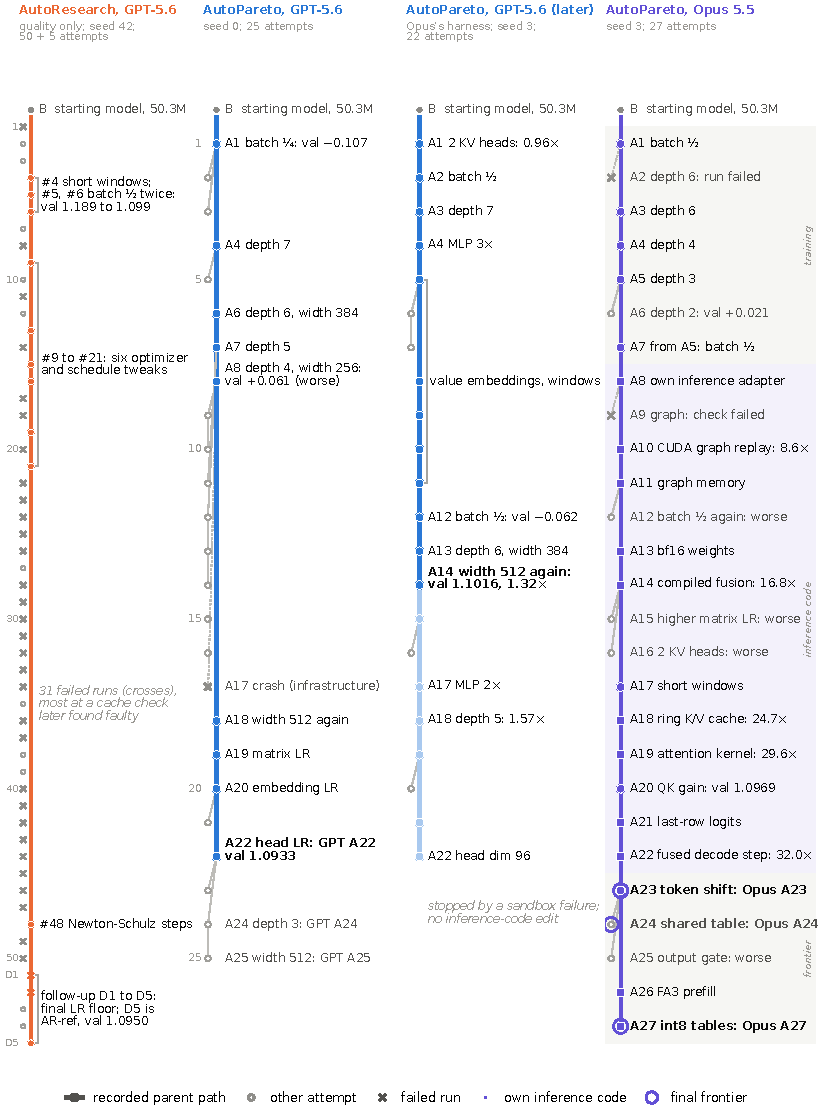
\includegraphics[width=\linewidth]{figures/cr_histories.pdf}
\caption{Every attempt of the four agent searches, one row per attempt in attempt order, with recorded parent links: AutoResearch (50 attempts and the 5-attempt follow-up D1 to D5; the scale is halved), GPT-5.6's seed-0 AutoPareto campaign (ending at GPT A22, with GPT A24 and A25 on a branch), GPT-5.6's later campaign under Opus's harness, and Opus. Opus's speed-ups are scored decode-only; validation BPB is comparable only within a column.}\label{fig:histories}\label{fig:lineagefull}
\end{figure}
\begin{table}[H]
\caption{Each step on the path to GPT A22 (seed 0, 300\,s, validation BPB): the edit derived from the frozen source, the measured outcome and change from the parent, and the opening words of the agent's recorded hypothesis, quoted verbatim. Steps after A18 move BPB by less than the pooled seed SD (\CRPooledSD). Full hypotheses are in the public registry.}\label{tab:apqpath}
\centering\scriptsize\setlength{\tabcolsep}{3pt}\renewcommand{\arraystretch}{1.1}% Generated by analysis/cr_v3.py from cr_evidence.json (seed-0 lineage) and lineage_edit_labels.json. Do not edit by hand.
\begin{tabular}{@{}l>{\raggedright\arraybackslash}p{2.35cm}rrr>{\raggedright\arraybackslash}p{6.0cm}@{}}
\toprule
Step & Edit (from the frozen source) & Val.\ BPB & $\Delta$ & Tokens (M) & Recorded hypothesis (opening words, verbatim) \\
\midrule
B & registered baseline: depth 8, width 512, batch $2^{19}$ & 1.2137 & & 90 & \\
A1 & batch $2^{19}\to2^{17}$ & 1.1063 & $-$0.1075 & 87 & ``Reducing total batch size from 2\textasciicircum{}19 to 2\textasciicircum{}17 will provide roughly four times as many optimizer updates within the fixed training window, \ldots'' \\
A4 & depth 8$\to$7 (width stays 512) & 1.1005 & $-$0.0058 & 97 & ``Reducing depth from eight to seven at width 512 will remove one full transformer block, materially improving cached decode speed and inference \ldots'' \\
A6 & depth 7$\to$6; width 512$\to$384 & 1.0978 & $-$0.0027 & 155 & ``Reducing depth from seven to six under the baseline aspect rule (width 512 to 384) will produce a substantially faster, lower-memory compatible \ldots'' \\
A7 & depth 6$\to$5 (width stays 384) & 1.0966 & $-$0.0012 & 177 & ``Reducing depth from six to five under the unchanged aspect rule will yield another large cached-decode speed and inference-memory gain, while the \ldots'' \\
A8 & depth 5$\to$4; width 384$\to$256 & 1.1573 & +0.0607 & 204 & ``Reducing depth from five to four under the unchanged aspect rule will preserve or improve validation BPB because the smaller model processes \ldots'' \\
A18 & aspect 64$\to$128; width 256$\to$512 & 1.0957 & $-$0.0616 & 160 & ``Increasing depth-four width from 256 to 512 will recover enough validation quality to establish a new high-quality frontier point while retaining the \ldots'' \\
A19 & matrix LR .04$\to$.035 & 1.0954 & $-$0.0003 & 160 & ``Reducing MATRIX\_LR from 0.04 to 0.035 on the depth-four width-512 model will improve validation BPB while preserving its high cached-decode rate and \ldots'' \\
A20 & embed LR .6$\to$.5 & 1.0934 & $-$0.0020 & 160 & ``Reducing EMBEDDING\_LR from 0.6 to 0.5 will combine with MATRIX\_LR 0.035 to further improve validation BPB on the depth-four width-512 model without \ldots'' \\
\textbf{A22} & head LR .004$\to$.0035 & 1.0933 & $-$0.0001 & 160 & ``Reducing UNEMBEDDING\_LR from 0.004 to 0.0035 will improve or preserve validation BPB while potentially recovering cached-decode speed, with architecture memory unchanged.'' \\
\bottomrule
\end{tabular}

\end{table}
The records also expose gaps between intent and execution. GPT-5.6's recorded intended changes for A7 and A8 predict widths 384, 320 and 256, but width rounding kept A7 at 384 and took A8 straight to 256.

\section{Questions a reader may ask}\label{app:faq}
\textbf{Is GPT A22 simply a worse model?} Per training token, yes (Table~\ref{tab:results}). Per GPU-second its held-out difference from AR-ref is not resolved (300\,s in E1, whose runs the 13-recipe test reuses), although the earlier seeds 0--2 re-runs found it slightly better on validation BPB (Table~\ref{tab:e1full}); meanwhile it is \CRParamReduction\% smaller, trains \CRSixGptTrainRatio$\times$ as fast and decodes \CRSixGptDecRatio$\times$ as fast with \CRSixGptMemRed\% less inference memory (Table~\ref{tab:verify}). Which matters depends on whether compute time or data is the scarce resource.

\textbf{Why not use a fixed-token contract from the start?} A fixed-time contract is the autoresearch standard and answers a practical question: the best model from a fixed amount of GPU time. It is not wrong, but it scores a program's throughput and its per-token quality together. A fixed-token contract isolates per-token quality but lets compute and update count vary. We report both.

\textbf{Why did every agent shrink the model?} Under 300\,s, BPB improves with more updates and tokens, and a smaller model gets more of both. The agents' hypotheses say so (Table~\ref{tab:reasoning}). E1 prices the trade for GPT A22: it trains \CREOneRho$\times$ faster but needs about \CREOneK$\times$ AR-ref's tokens for equal quality, so at 300\,s the two roughly cancel. Opus's recipes would need more than \CRMTKBound$\times$ AR-ref's tokens, about their speed advantage, and in the pre-registered 13-recipe test they do not differ resolvably from AR-ref at 300\,s (95\% CIs span zero; Table~\ref{tab:paired6}).

\textbf{Does a 201.3M-token budget favour the larger model?} It is about 2.3$\times$ AR-ref's own 300\,s exposure and within 3\% of Opus's. E1 also ran 88.6M and 157.3M tokens, the first matching GPT A22's discovery exposure, and GPT A22 is worse at every budget (Figure~\ref{fig:e1}). The other recipes ran one matched budget, so their gap's dependence on it is untested.

\textbf{Does E1 prove that exposure is the only cause?} No. E1 shows that at equal tokens and updates GPT A22 is worse, on the same seeds and data, and its exploratory split attributes the 300\,s result to extra tokens offsetting a weaker architecture. Tokens and updates move together, and architecture and optimizer edits are bundled, so finer causes are not separated.

\textbf{Are three seeds enough?} For the matched-token gap, yes: \CREOneMatchedLoAbs--\CREOneMatchedHiAbs{} held-out BPB against a within-recipe seed SD of at most \CREOneMaxSD, on all \CREOnePairs{} seed--budget pairs, and the panel result replicates on other seeds and another A40. In the 13-recipe test all \CRSixTokWorseCount{} matched-token gaps to AR-ref are resolved per comparison, each worse on all three seeds, and \CRSixBonfTok{} remain resolved after a Bonferroni adjustment for the 12 comparisons (Table~\ref{tab:paired6}). For the slope of the gap with tokens, or to show equivalence at 300\,s, no.

\textbf{Did Opus game the decode metric?} It stayed within the permitted surface: the adapter had to compute the same outputs, and every variant passed the correctness checks on the 64- and 256-token prefixes they cover, two runs (Opus A24 with a plain K/V cache) only after FP32 adjudication. Those checks do not reach the timed window after the 1{,}024-token prompt. The 13-recipe test closed this gap for the submitted recipes: in all \CRSixCorrectRuns{} runs, \CRSixAgreePct\% of the generated tokens (all 8 prompts, positions 1{,}024 to 1{,}151, past the ring caches' wrap) equal the uncached model's greedy choice and the other \CRSixNearTies{} are near-ties within the registered 0.25-logit bfloat16 tolerance; none is a hard mismatch (Appendix~\ref{app:repro}). Its records describe graph replay as a fix for launch-bound decode and note the prefill cost (Table~\ref{tab:reasoning}), so it was the metric's definition, not a rule violation, that rewarded the placement. We report decode-only and end-to-end speed side by side and recommend prefill-inclusive scoring.

\textbf{Is the Codex--Opus comparison fair?} The arms share the baseline, seed, prompt bytes, output schemas, contract, Pareto rule and the hook for the agent's own inference code (Appendix~\ref{app:access}). They differ in reasoning setting (high vs xhigh), agent-call timeout (600 vs 900\,s from Opus A10), isolation, harness repairs and attempt count (\CRCxAttempts{} vs \CROpAttempts), and each ran one seed. At \CRCxAttempts{} attempts each the best validation BPBs are \CRCxBestBPB{} and \CROpBestTwentyTwo. We draw no agent ranking. The arms show the same exposure strategy and supply recipes for retraining.

\textbf{Does the Opus extension to \CROpAttempts{} attempts change anything?} No. Its best validation BPB (\CROpBestFrozen) came within the frozen first 25 attempts. The frozen frontier (\CROpFrontierFrozen) shares Opus A23 and A24 with the retrained set, and the third retrained recipe, Opus A27, matches Opus A23's held-out gap to AR-ref to three decimals (Table~\ref{tab:results}).

\textbf{Could the time-to-token mapping handicap Opus's recipes?} The mapping changed only driver lines (clock, stop, progress). Model and optimizer code stayed byte-identical. The 201.3M tokens and 1{,}536 updates are within 3\% of Opus's own 300\,s runs (\CROpTokLo--\CROpTokHi M tokens, \CROpUpdLo--\CROpUpdHi{} updates), so its recipes were scored at almost the exposure they were tuned for, and an AR-ref drift control reproduced E1 within \CRMTDriftAbs{} BPB.

\textbf{Were the reported recipes cherry-picked?} The funnel and its dates are in Table~\ref{tab:funnel}: the representative rule predates the first attempt, the four-role selector preceded the seeds 0--2 confirmation, and the panel was assembled after it. A full-size candidate (exp 109) was never confirmed. AR-ref replaced exp 65, which failed a cache-correctness check under a reference later judged faulty, and their fixed-time re-runs do not differ resolvably (\CRFixedSixtyFive{} and \CRFixedSixtyEight). E1, the Opus retraining, the ablations and the 13-recipe test were pre-registered; the Opus retraining covers its whole frontier, and the 13-recipe test retrained the best recipe of every approach except GPT-5.6's later campaign, including the three classical optimizers never retrained before.

\textbf{Does this transfer to larger models or other GPUs?} Untested: one GPU type and recipes of 18--50M parameters.

\section{Disclosure Statement}
% Revision 6 (Claude draft for the author's final review). The two checkbox declarations of earlier
% versions were removed at the author's request: the public workshop page does not ask for them in the
% PDF. If the Overleaf template or the OpenReview instructions require them, restore them from
% camera_ready/source_before_revision6/main.tex.
\humanauthor[Disclosure r6]{This paper involved AI in three distinct roles, and the records keep them apart.

\textbf{Autonomous research agents.} The scientific changes searched in this paper were proposed by research agents: GPT-5.6 in the original experiments and the extended Codex arm, and Claude Opus 5.5 in the extended Opus arm (\S\ref{sec:agent}). Interventions whose authorship cannot be reconstructed are excluded from claims of autonomous contribution (\S\ref{sec:interventions}).

\textbf{AI assistants.} The author used Claude (Opus 5.5, through Claude Code) as a coding, analysis and writing assistant, in sessions separate from every research-agent campaign. Under plans the author approved, it wrote the code for and ran the pre-registered camera-ready experiments (E1, the Opus retraining, the inference ablations and the 13-recipe test), wrote the analysis and figure scripts, and drafted and edited manuscript text, including suggested wording for Part~2. It belongs to the same model family as the Opus research agent but had no role in that agent's proposals. AI coding assistants also carried out some of the human interventions of \S\ref{sec:interventions} at the author's instruction.

\textbf{Human author.} The author designed the study, chose its objectives, contracts and comparators, made or approved every intervention, directed the verification and is responsible for the submitted claims. Authorship of this submission is human only.}

\bibliographystyle{plainnat}
\bibliography{references}
\end{document}
